\documentclass[12pt]{article}

\usepackage{amsmath, amsthm, amsfonts, enumitem, graphicx, subcaption, cleveref, tabularx, xpatch, imakeidx, setspace, mathptmx, titlesec, fancyhdr, etoolbox, tocloft, float, lipsum, amssymb, algorithm, algpseudocode}
\usepackage[font=small, singlelinecheck=off]{caption}
\usepackage[backend=biber,style=numeric]{biblatex}
\usepackage[a4paper,top=3cm,bottom=2.5cm,left=2.5cm,right=2.5cm]{geometry}
\makeindex

\addbibresource{src/bib/references.bib}

% TIPOGRAPHY
% Page settings
\pagestyle{fancy}
\fancyhf{}
\fancyfoot[C]{\thepage}

% Line spacing
\onehalfspacing

% Paragraph indent
\setlength{\parindent}{0.7cm}

% Chapter and section titles
\titleformat{\chapter}[display]{\bfseries\Huge}{\chaptername\ \thechapter}{20pt}{\bfseries\LARGE}
\titleformat{\section}{\normalfont\Large\itshape}{\thesection}{1em}{}

% Blockquote setup
\newenvironment{blockquote}{\begin{quote}\onehalfspacing\fontsize{11}{13.2}\selectfont}{\end{quote}}

% Footnotes
\renewcommand{\footnotesize}{\fontsize{10}{12}\selectfont}
\setlength{\footnotesep}{\baselineskip}
\appto\footnotesize{\singlespacing}

% CUSTOM COMMANDS
\newcommand{\meqref}[1]{Eq.\ref{#1}}
\newcommand{\mfigref}[1]{Fig.\ref{#1}}
\newcommand{\mtabref}[1]{Tab.\ref{#1}}
\newcommand{\mappendixref}[1]{Appendix \ref{#1}}
\newcommand{\indfunc}[1]{\textit{\textbf{1}}_{#1}}
\newcommand{\midcaption}[1]{
    \captionsetup{justification=centering}
    \caption{#1}
}
\makeatletter
\xpatchbibmacro{textcite}{%
  \printnames{labelname}%
}{%
  \printfield[citetitle]{labelname}%
}{}{}
\DeclareCiteCommand{\fancycite}
  {\usebibmacro{prenote}}
  {\textit{\printnames{labelname}%
   \ifnum\value{citecount}=1 \printtext{ et al.} \fi%
   (\printfield{year}) \textsuperscript{\printfield{labelnumber}}}}
  {\multicitedelim}
  {\usebibmacro{postnote}}
\makeatother
\makeatletter
%\DeclareFieldFormat{labelnumber}{\textit{\mkbibsuperscript{#1}}}
\DeclareCiteCommand{\ucite}
  {\usebibmacro{prenote}}
  {\textsuperscript{\textit{\printfield{labelnumber}}}}
  {\multicitedelim}
  {\usebibmacro{postnote}}
\makeatother

\begin{document}

\title{Properties and Implementation of Sequential Expansion of Latin Hypercube Sampling for Simulation Design}
\author{Crespi Alessandro, Gerosa Davide, Boschini Matteo}
\date{July, 2024}
\maketitle

\tableofcontents
\pagebreak

\begin{abstract}
Lorem ipsum dolor sit amet, consectetur adipiscing elit. Proin luctus finibus euismod. Quisque purus mauris, mollis sed tellus quis, congue hendrerit eros. Aliquam tempus suscipit risus non viverra. Ut pharetra mollis ante, sit amet vestibulum augue laoreet eget. Nunc tincidunt ex sit amet rutrum euismod. Maecenas feugiat, mi aliquam semper rutrum, purus justo imperdiet massa, sed feugiat leo libero sit amet sapien. Mauris sit amet sem rhoncus, hendrerit nunc sed, sagittis felis. 
\end{abstract}


\section{Introduction}
Simulation design is a branch of Statistics that studies ways to build better simulations, intended as tools for enhancing the comprehension of phenomena, which have become widely used in mathematics, physics, economics, mechanics, and every scientific field as experimental tools for proofing theories, interpolating real sampled values, and, more generally, generating predictive models that try to explore uncharted traits, features, and peculiarities, perhaps intuitively or roundly developed in the early stages of the study of a specific problem.

Since the advent of hybrid mechanical-electrical programmable calculators such as IBM's machines, the first of their kind to be really useful in engineering, scientists have them involved in heavy computations for experiments. Following, in 1969, the Kennar and Stone's Computer Aided Design for Experiments (CADEX)\ucite{kennard1969} proposal for computer-driven experiments has led to spread up a broad variety of Computer-based simulation methods.

Eventually, computer-based simulations are a set of strategies that benefit from mathematical modelling techniques based on discrete known points placed in a limited parameter space, hereafter samples, and the computer programmability advantage has been used to design, shape and enhance a specific subset of samples that satisfy the desired properties, hereafter sample sets. 

The general concept of computer simulation has been defined in the past few decades, it's based on the following key ideas: taking into account a desired behavior $ F $ the experimenters have an interest in, F has to be explored through its $ N $ real parameter space; the algorithm takes randomly samples from a standard $ N $-dimensional hyperspace $ \Omega $ and arranges the sample set for the simulation; afterwards, the simulation is carried out by evaluating $ F $ over the sample set and eventually producing a so-called surrogate model. The class of algorithms meant to implement this abstraction is commonly named as Sampling Methods.

A critical consideration when evaluating sampling methods is the trade-off between exploration and exploitation. An exploration-oriented sample set maximizes the simulation skill of seeking key features over the studied behavior. Exploration has been depicted as a model-free practice, so that it does not base its own actions on the model (behavior) evolution or any other on-site response. On the other hand, exploitation is an auxiliary mechanism that aims to better assist the simulation by deploying samples in strategic placements that prevent exploration from exceeding the prediction surrogate made upon a key region (such as overshooting an optima or mismatching a discontinuity for a steep slope).

The most iconic sample method for simulations is obviously the pseudo-random sampling, lightened of every other criteria, namely the Monte Carlo Sampling or MCS (\fancycite{metropolis1987})  which it has been proposed as fundamental design of sampling methods. Quasi-Monte Carlo methods are a class of sampling algorithms based on Monte Carlo, indeed, but without a proper random drawing of sample points from the parameter space, instead, points are sequentially extracted in order to satisfy one or multiples criteria as best as the computational time required remains acceptable.
 
Many criteria have been theorized and tested; each of them has its own best scenario, which it'd be better to apply to. An updated, summarized list of the most remarkable ones is shown and commented in section \cref{subsec:lhs_properties} in \cref{tab:remarkable_criterions}. As per the interest of this paper, the reader is going to learn about the space-filling class of criteria and the one-projection property (also known as non-collapsing property or projective property); the latter has been widely known because of the Latin Hypercube Sampling (LHS), topic of this research and explained afterwards. The space-filling design of points measures the quality of a sample set to be spread evenly across an hyperspace; the way space-filling is defined determines the final aspect of the sampling. On the other hand, a sample set, in $P$-dimensional space, admits the one-projection property if and only if each projection of every sample $x$ on a specific axis does not overlap onto each other's interval $I_j$. These $I_j$ intervals are well-known fixed-width slices of the limited volume of parameter space taken into examination (e.g., a volume $[0,1)^N$ ) and the number of intervals is equal to the number of samples taken. So, the non-collapsing property prevents samples to fall into a busy "private space" (which has been occupied by another sample). Furthermore, given that the number of intervals and the size of the sample set is equal, it does ensure there are no empty intervals across the parameter space.

The authors used to work with sampling methods for simulation design, more likely LHS designs, in Astrophysics related experiments, such as simulating black hole binary systems collapsing, which obviously requires a massive amount of computational time and many different parameters. The authors often experienced difficulties predicting how long it would take to run a full simulation given $N$ known sampling points in a $P$-dimensional space. This situation forces them to reserve more machine time on a shared company supercomputer for experiments than they really need. In order to better spend the reserved machine time left after the execution of the first run of sampling points, the authors designed an algorithm that adds up points to the previous LHS' sample set and another set of samples that has been drawn by the expansion algorithm in order to preserve the non-collapsing property of both sample sets together.

The authors of this paper propose a algorithm called "Expansion of an LHS" that, indeed, takes a already existing Latin Hypercube Sampling' sample set and propose a new set of points samples in the same parameter hyperspace which are suppose to maximize the non-collapsing property of the samples altogether. 
The original sample set is referred as "starting set" and the add-on samples as "expansion set". The whole sample set joined together by both is called "expanded simulation".

The paper is structured as follows: \cref{sec:lhs} yields a Latin Hypercube Sampling brief history and formal definition; in \cref{sec:lhs_expansion} is shown the research results and discussion of the expansion task issued; \cref{sec:conclusions} [...].

\section{Latin Hypercube Sampling}
\label{sec:lhs}
\subsection{What is an LHS?}
\label{subsec:what_is_an_lhs}
According to the Handbook of Computational Designs (2nd edition, 2006) \ucite{colbourn2006}, the first appearance in history of the "Latin Square" has to be attributed to the Korean mathematician Choi Seok-jeong, who described it, using modern terminologies, as a $N \times N$ matrix (the square) with $N$ distinct symbols, appearing $N$ times each but precisely once per type for each row and column. The suffix "Latin" has been inspired by the efforts that Leonhard Euler has put into this topic while defining a general theory for Latin Squares \ucite{wiki_latin_square} and using Latin letters as symbols to fill the square up with. See Fig.1 for an example with 4 objects.

\begin{figure}[h]
    \centering
    \begin{subfigure}[b]{0.45\textwidth}
        \centering
        \vtop{
        	\vspace{0pt}
        	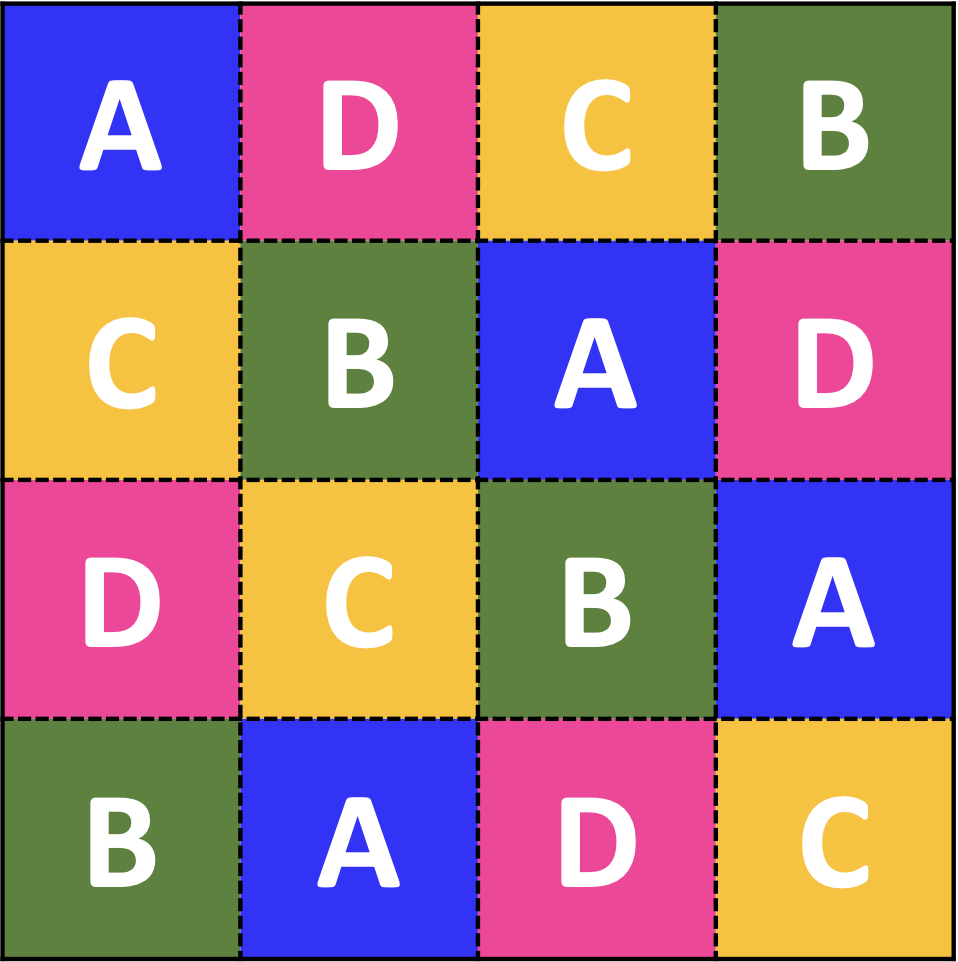
\includegraphics[width=\textwidth]{src/imgs/latin_square_letters_and_colours.png}
        	%\captionsetup{}
        	\caption{A Latin 4x4 Square with 4 distinct symbols, both letters or colors either, arranged so that no letter occurs more than once in a row or a column}
        	\label{fig:latin_square_a}
        }
    \end{subfigure}
    \hspace{0.05\textwidth}
    \begin{subfigure}[b]{0.45\textwidth}
        \centering
        \vtop{
        	\vspace{0pt}
        	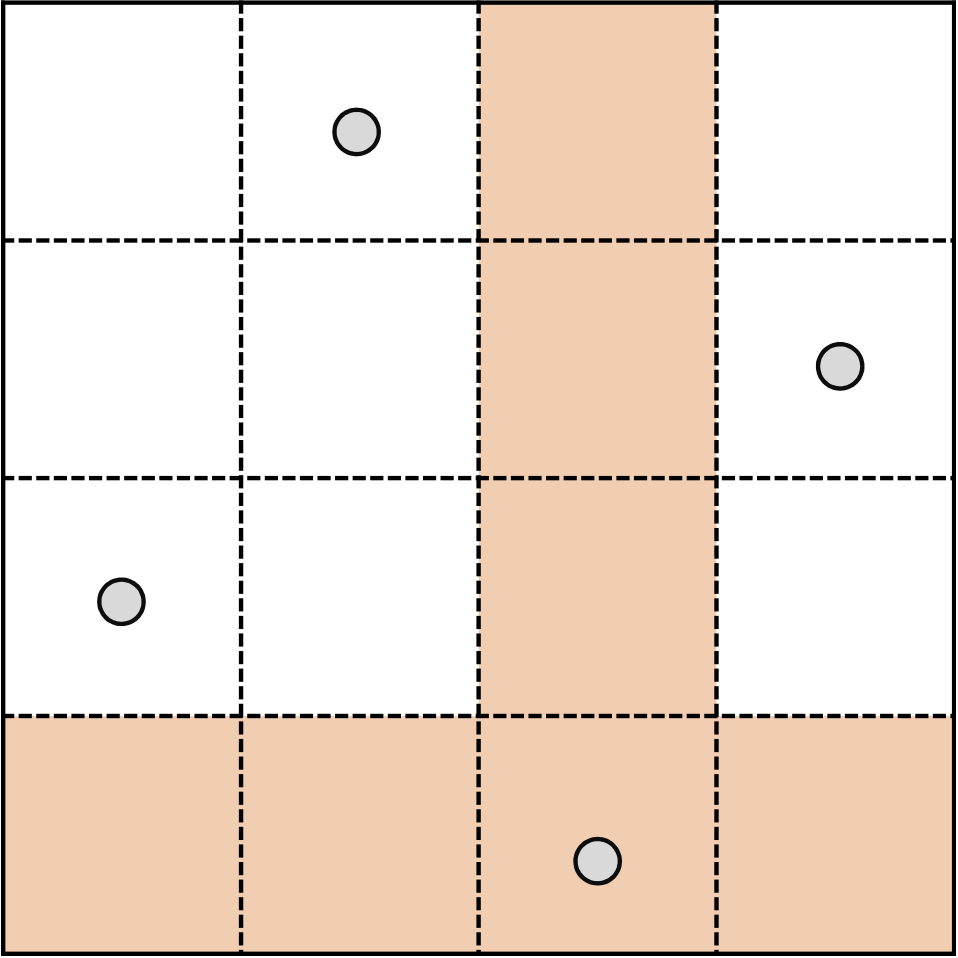
\includegraphics[width=\textwidth]{src/imgs/latin_square_skeleton.png}
        	\caption{The skeleton of (a) Latin Square highlighting only the D (or PINK) symbol positions, it's easily noticeable how the positions does not overlap onto each other's row and column both}
        	\label{fig:latin_square_b}
        }
    \end{subfigure}
    
    \midcaption{The images were kindly taken from \fancycite{sheikholeslami2017}}
    \label{fig:latin_square}
\end{figure}

Per the interest of this paper, which doesn't aim to study how the symbols behave with each other and several algebraic combinatorics considerations, and for sake of clarity, the $N$ number of distinct symbols factor is not taken into account anymore. Instead, it has been considered a sole symbol, hereafter "sample", which has to obey the "do not cross into each other's row and column", hereafter non-collapsing property. The sample must occur in the hyper-matrix exactly $N$ times.

Generally, we can speak of "Hypercubes" by transposing the classic 2-dimensional matrix concept (depicted as a grid in Fig.1a) into a more complex multidimensional matrix where $N$ samples are placed such that each one lies exactly once on each fiber (in literature, a "fiber" of a multidimensional matrix is the general term for a one-dimensional substructure in any dimension (mode) of a tensor. e.g. In a 2D matrix, the fibers of the first and second dimensions are respectively "rows" and "columns").

The modern approach of LHS is not supposed to place symbols in matrices but, instead, attempts to place $N$ samples on hyperspaces that represent the examined parameter space of the interested model, where each axis is associated with a different parameter. The parameter hyperspace has a limited span, which is the hyper-volume $[0,1)^P$, commonly used in literature, which represents, again, a hypercube. However, some texts use a different standard, and they let the parameter space take place in a $[-1,1)^P$ hypercube. Every parameter axis is sliced into smaller consecutive intervals of width $\frac{1}{N}$ that consequently depict the sub-region where each coordinate of the points is sampled randomly. In anticipation for further definitions, we provide a indexing system for intervals; in any dimension of the hypercube with $N$ intervals, for each $j$ from 0 to $N-1$, the j-th interval's boundaries are:
\begin{equation}
\label{eq:interval_index}
I_j = \Big[\frac{j}{N}, \frac{j + 1}{N}\Big)
\end{equation}
for further usage, the right term $\frac{j + 1}{N}$ of the interval was called \textit{frontier of the j-th interval} which is shared with the left hand term of $I_{j+1}$. 
With no loss of generality, the examples and considerations designed by the authors of this paper assess the random distribution to be uniform in all intervals. The uniformly distributed samples can be transformed by associated transformation functions for any other distribution (e.g., a Gaussian distribution).

\subsection{How to build a Latin Hypercube Sample Set}
\label{subsec:how_to_lhs}
In this section it has been marked out mathematically the construction of an LHS sample. This description is widely used for introducing the topic on many textbooks and lectures and it takes inspiration from the work of X.Kong at al.\ucite{kong2017}.
Let $S = \{S_1, S_2, ..., S_N\}$ be the Latin Hypercube sample set with $N$ number of samples, where for each $S_i$ its cardinality is $P$ number of dimensions. It is comfortable to use the matrix representation $S_{ij}$ whereof rows are the i-th sample and columns, instead, represents the projection of every sample on each j-th dimension. Then, we introduce the sorted index matrix $A = \{A_{ij} = j - 1\}$ as a tool for trace the intervals index (starting from zero), its purpose will be clearer soon. \\
Given an $A$ index matrix, the preliminary design matrix S is given by: 

\begin{equation}
\label{eq:Sij_def}
S_{ij} = \frac{a_{ij} + u_{ij}}{N}
\end{equation}

where $u_{ij}$ is a uniform distributed variable U[0,1). This preliminary design has the peculiarity to have the samples always placed on the diagonal of the hypercube $[0,1)^P$. Now the index matrix come into use, typically shuffling the original $A$ we attain $B = \{b_{ij}\}$ random permutation, which plugging it  into \cref{eq:Sij_def} describe the uniform random variable $S_{ij}$ living inside the statistical bin identified by the interval index $b_{ij}$. We explicitly write down the uniform random variable $S_{ij}$ involving \cref{eq:interval_index} boundaries for the ij-th interval as well: 
\begin{equation}
\label{eq:rand_variable_Sij}
S_{ij} \text{ $\sim$ } U\Big[\frac{b_{ij}}{N}, \frac{b_{ij} + 1}{N}\Big)
\end{equation}

\subsection{Grade of a Sample Set}
\label{subsec:lhs_grade}
For the purpose of this research, the authors introduced a tool meant to measures how much a Monte Carlo sample set is close to a Latin Hypercube one, namely "grade of a sample set". This metric \meqref{eq:grade} has been designed to reduce the sampling $S$ of $N$ elements to an index between 0 and 1 (percentage), when it's compared against the $P$-dimensional hypercube sectioned for the LHS that would have covered it if $S$ was generated to fulfill the one-projection property.

\begin{equation}
\label{eq:grade}
gr(S) = \frac{\sum^P_{j=1}\sum^N_{q=1} min(\sum^N_{i=1}\indfunc{[\frac{q-1}{N}, \frac{q}{N})}(S_{ij}), 1)}{P \cdot N}
\end{equation}

where $\indfunc{}$ is the indicator function (see \mappendixref{appendix:indicator_function}), the variable $q$ is another way to represent the sorted index matrix $A = \{a_{ij} = j \}$ for a more immediate comprehension. The formula has meant to compute the arithmetical average of the presence (with numerical value 1) of the projection of every sample in each interval for each dimension. The use of the $min$ operator states that the presence of several samples' projections in a specific interval $q$ doesn't weight up the whole term, which would be at most 1 even if multiple sample lies in $q$. Hence, the grade formula ignores the overlapping samples onto the same interval, hereafter only \textit{overlaps}. 

\subsection{Additional properties (Work in progress)}
\label{subsec:lhs_properties}
In this section, the reader will deal with the idea of adding properties that could improve the accuracy - or the quality in other terms - of the surrogate model produced when the simulation is consumed.
A well known issue with LHS designs is well depicted in \mfigref{fig:diagonal_poor_design}. It's obvious that it must be considered a poor simulation design for the most of the experiments. In fact, every really distributed implementation of LHS adds some peculiar properties to the design. We can highlight two superclasses of properties which LHS may be joined with: model-free properties and model-based properties.


\begin{figure}[h]
    \centering
    \begin{subfigure}[b]{0.45\textwidth}
        \centering
        \vtop{
        	\vspace{0pt}
        	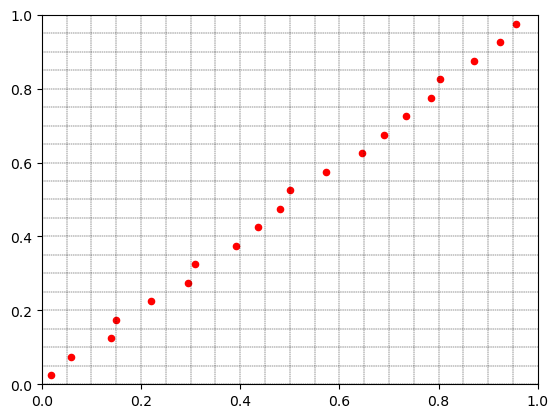
\includegraphics[width=\textwidth]{src/imgs/diagonal_poor_design.png}
        	\caption{A poor Latin Hypercube sampling in 2 dimension despite it fulfill the one-projection rule. This experiment shows how simple LHS can be insufficient to achieve a good simulation.}
        	\label{fig:diagonal_poor_design}
        }
    \end{subfigure}
    \hspace{0.05\textwidth}
    \begin{subfigure}[b]{0.45\textwidth}
        \centering
        \vtop{
        	\vspace{0pt}
        	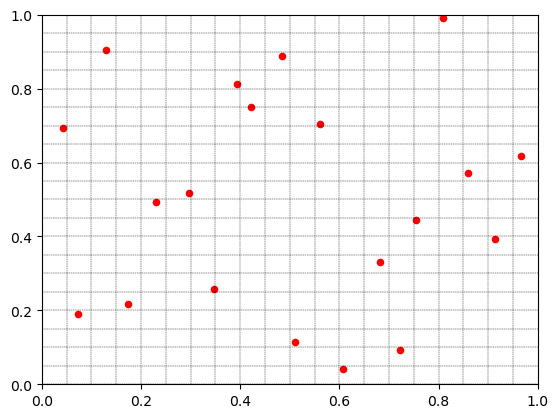
\includegraphics[width=\textwidth]{src/imgs/good_design.png}
        	\caption{This sampling has been generated using scipy LHSSampler utility class. The sample set bears random permutations of coordinates to lower the centered discrepancy. \ucite{scipy_lhs}}
        	\label{fig:good_design}
        }
    \end{subfigure}
    
	\midcaption{}
    \label{fig:latin_square}
\end{figure}

\subsubsection{Model-free and model-based simulation designs}
\label{subsubsec:model_free_model_based}
As the names may suggest, the latter implies the experimental design to involve some the peculiarities of the function to evaluate e.g. the shape that is expected, the initial or boundaries conditions, any well known critical region. Given that this approach is knowledge-driven, "What do we already know about?", can knock down pretty much the computational time required for the whole experiment with eventually high accuracy, but it can be equally easy that results may be deformed, based on assumptions that may prove wrong later, or make hard any further effort from other scientists to retake the experiment and confirm the results if the assumptions are not completely clear.
On the other hand, the model-free is the formal way to depict a fully independent sampling of the parameter space from the experiment which it has been designed for. Because of not many criteria have been left, all of the properties in this class are based on inter-element relationships, which convey that for each of them has a heuristic meant to quantify how much each sample is well-placed among the others. The shorthand for such a class of criteria is \textit{space-filling properties}.

Beside the many interesting considerations and suggestions that the model-based class of criteria has to offer to mathematicians, the space-filling properties has highly excited the experimenter community through the decades, producing creative and curious features that the samples could experience among each others. A very short list of the most representative ones is shown in \mtabref{tab:remarkable_criterions}. The most simple one is the [L2? phi di P?] criterion where the assumed metric is the Euler distance between each point in the hyperspace. The non-trivial issue comes along with the computational effort necessary to run through the search tree generated by the maximin (or minimax?) algorithm.

By the way, the characteristic non-collapsing property of the LHS itself is actually a space-filling property. It ensures that, for example, the average distance between the consecutive projections of a group of 3 samples on the same axis is at least 1/2 distance units and at most 3/2 d.u.

\begin{table}[h]
	\label{tab:remarkable_criterions}
    \centering
    \begin{tabularx}{\textwidth}{X X X X} 
        \textbf{Authors} & \textbf{Year} & \textbf{Algorithm} & \textbf{Criteria} \\
        \hline
        \text{Audze and Eglajs} & 1977 & \text{Coordinates exchange} & \text{Potential energy} \\
    \end{tabularx}
    \caption{ Riempio la tabella piano piano che leggo i paper. Ho visto che molte ricerche su LHS usano dare una cronologia sull'utilizzo dei criteri utilizzati throught history}
\end{table}

\section{Expansion of a Latin Hypercube Sampling}
\label{sec:lhs_expansion}
The LHS paradigm's ability to implement several criteria over a rigorous grid, which forms the basis for the sequential creation of samples, has made it frequently utilized in engineering environments for surrogate manufacture of complex systems - see also \cref{subsec:lhs_properties}. For example, the LHS is used in hyperparameter tuning/optimization of Machine Learning models (\fancycite{koch2018}), environmental and water system analysis (\fancycite{sheikholeslami2017}), structural reliability analysis (\fancycite{olsson2003}) and many others.

As happens with every helpful technology, researchers and scientists have attempted to improve the LHS capability. As previously stated, add criterions first. Then, by rethinking the foundations of the algorithm. The reader has to acquaint that our Monte Carlo pseudo-random distribution, namely the Latin Hypercube technique, widely implemented, was labeled in literature as a \textit{one-stage} algorithm. The fact that all samples are distributed and assessed "on the first run" bestows this adjective. It's relevant to clear out that the actual creation and propagation of points is not properly implemented as the resulting of a lone drawing of \meqref{eq:rand_variable_Sij} random variables, but instead it's a sequential drawing of points - might be a parallel drawing of several ones for optimization reasons, but it hasn't been a topic of this research - which the newest one has to be pulled out from a pool of optimal candidates in order to improve the criteria applied, given a desired $N_1$ number of samples, such as Maximin space-filling distance. The feature "one-stage" highlights that it could be possible to have many more "stages" of the algorithm. It's a game of perspectives: inside a current stage, the policy for drawing a fixed number of data points is aimed at pulling out point given the other ones; instead, a multistage policy is related to a more evolutionary approach, aiming to enhance the sample set stage by stage. Manipulate an already instantiated LHS may sounds difficult because LHS hasn't been designed for adding points - or, at least, it's not supposed to consider it. Indeed, it is reasonable to assess that by adding points, one by one, over a full grid of $N_1$ intervals of an LHS, and then reshaping such a grid in $N_2 > N_1$ intervals, should soon lead to collisions (overlaps), which represents an issue that scientists had to deal with which suggest noticeable solutions - see \cref{subsec:multistage_task} for more.

The process that embodies the evolution from a precursor LHS to his next-stage has been called \textit{Expansion} by the authors; the resultant of the expansion process is the so-called \textit{expanded set}. Please refer to \cref{subsec:expansion_theory} for the visual explanation of expansion.

Along this section, the authors used to refer several times to the expansion process without precising how the new samples are going to be placed, the actual process is described in section \cref{subsec:expansion_theory}.

\subsection{The task of multistaging sampling}
\label{subsec:multistage_task}
Concerns regarding the consistency of the one-projection property, which is valid for one-staged setups, are raised by the multistage approach. \mfigref{fig:example_overlaps} depicts an experiment carried out upon scipy's $X$ with LHS distribution configured with $N_1 = 10$ samples displayed over its appropriate grid of $N_1$ intervals per dimension. The experiment consists in evaluating the behavior of the fixed $X$ while the grid is "growing" - intended as creating a brand new grid with  a greater number of intervals - one by one for three times. 
Light grey-colored rows and columns are vacant, meaning that no projections are located there; rows and columns marked in red indicate the locations of overlaps. After the first add-on (\mfigref{fig:example_overlaps1}), the grid shows two overlaps in row \#3 and in column number \#3 as well; the next stage (\mfigref{fig:example_overlaps2}) shows overlaps too, four in total, more than before. In the end, \mfigref{fig:example_overlaps3} has no overlaps at all. The read might have had an hunch about the distribution of occurrences of overlaps if kept growing the grid, such a distribution should be based on the initial sample set. The authors discuss about this topic later in [section does not exist yet].

Regarding the LHS directive, the multistage experiment proposed shows that growing the interval grid could lead to a general downgrade the one-project (\mfigref{fig:example_overlaps2} and \mfigref{fig:example_overlaps3}) or could give a new opportunity to fill the new empty space with a set of brand new samples without compromise the whole set optimality. 

The resulting sample set $Z$ of the expansion process which takes place upon a well-formed LHS of $N$ elements - hereby \textit{perfect LHS} - over a growing $M+N$ grid is called \textit{perfect expansion} if and only if $Z$ reaches the \textit{upper expanded grade limit} \meqref{eq:expanded_grade}.

\begin{figure}[]
    \centering
    \begin{subfigure}[b]{0.49\textwidth}
        \centering
        \vtop{
        	\vspace{0pt}
        	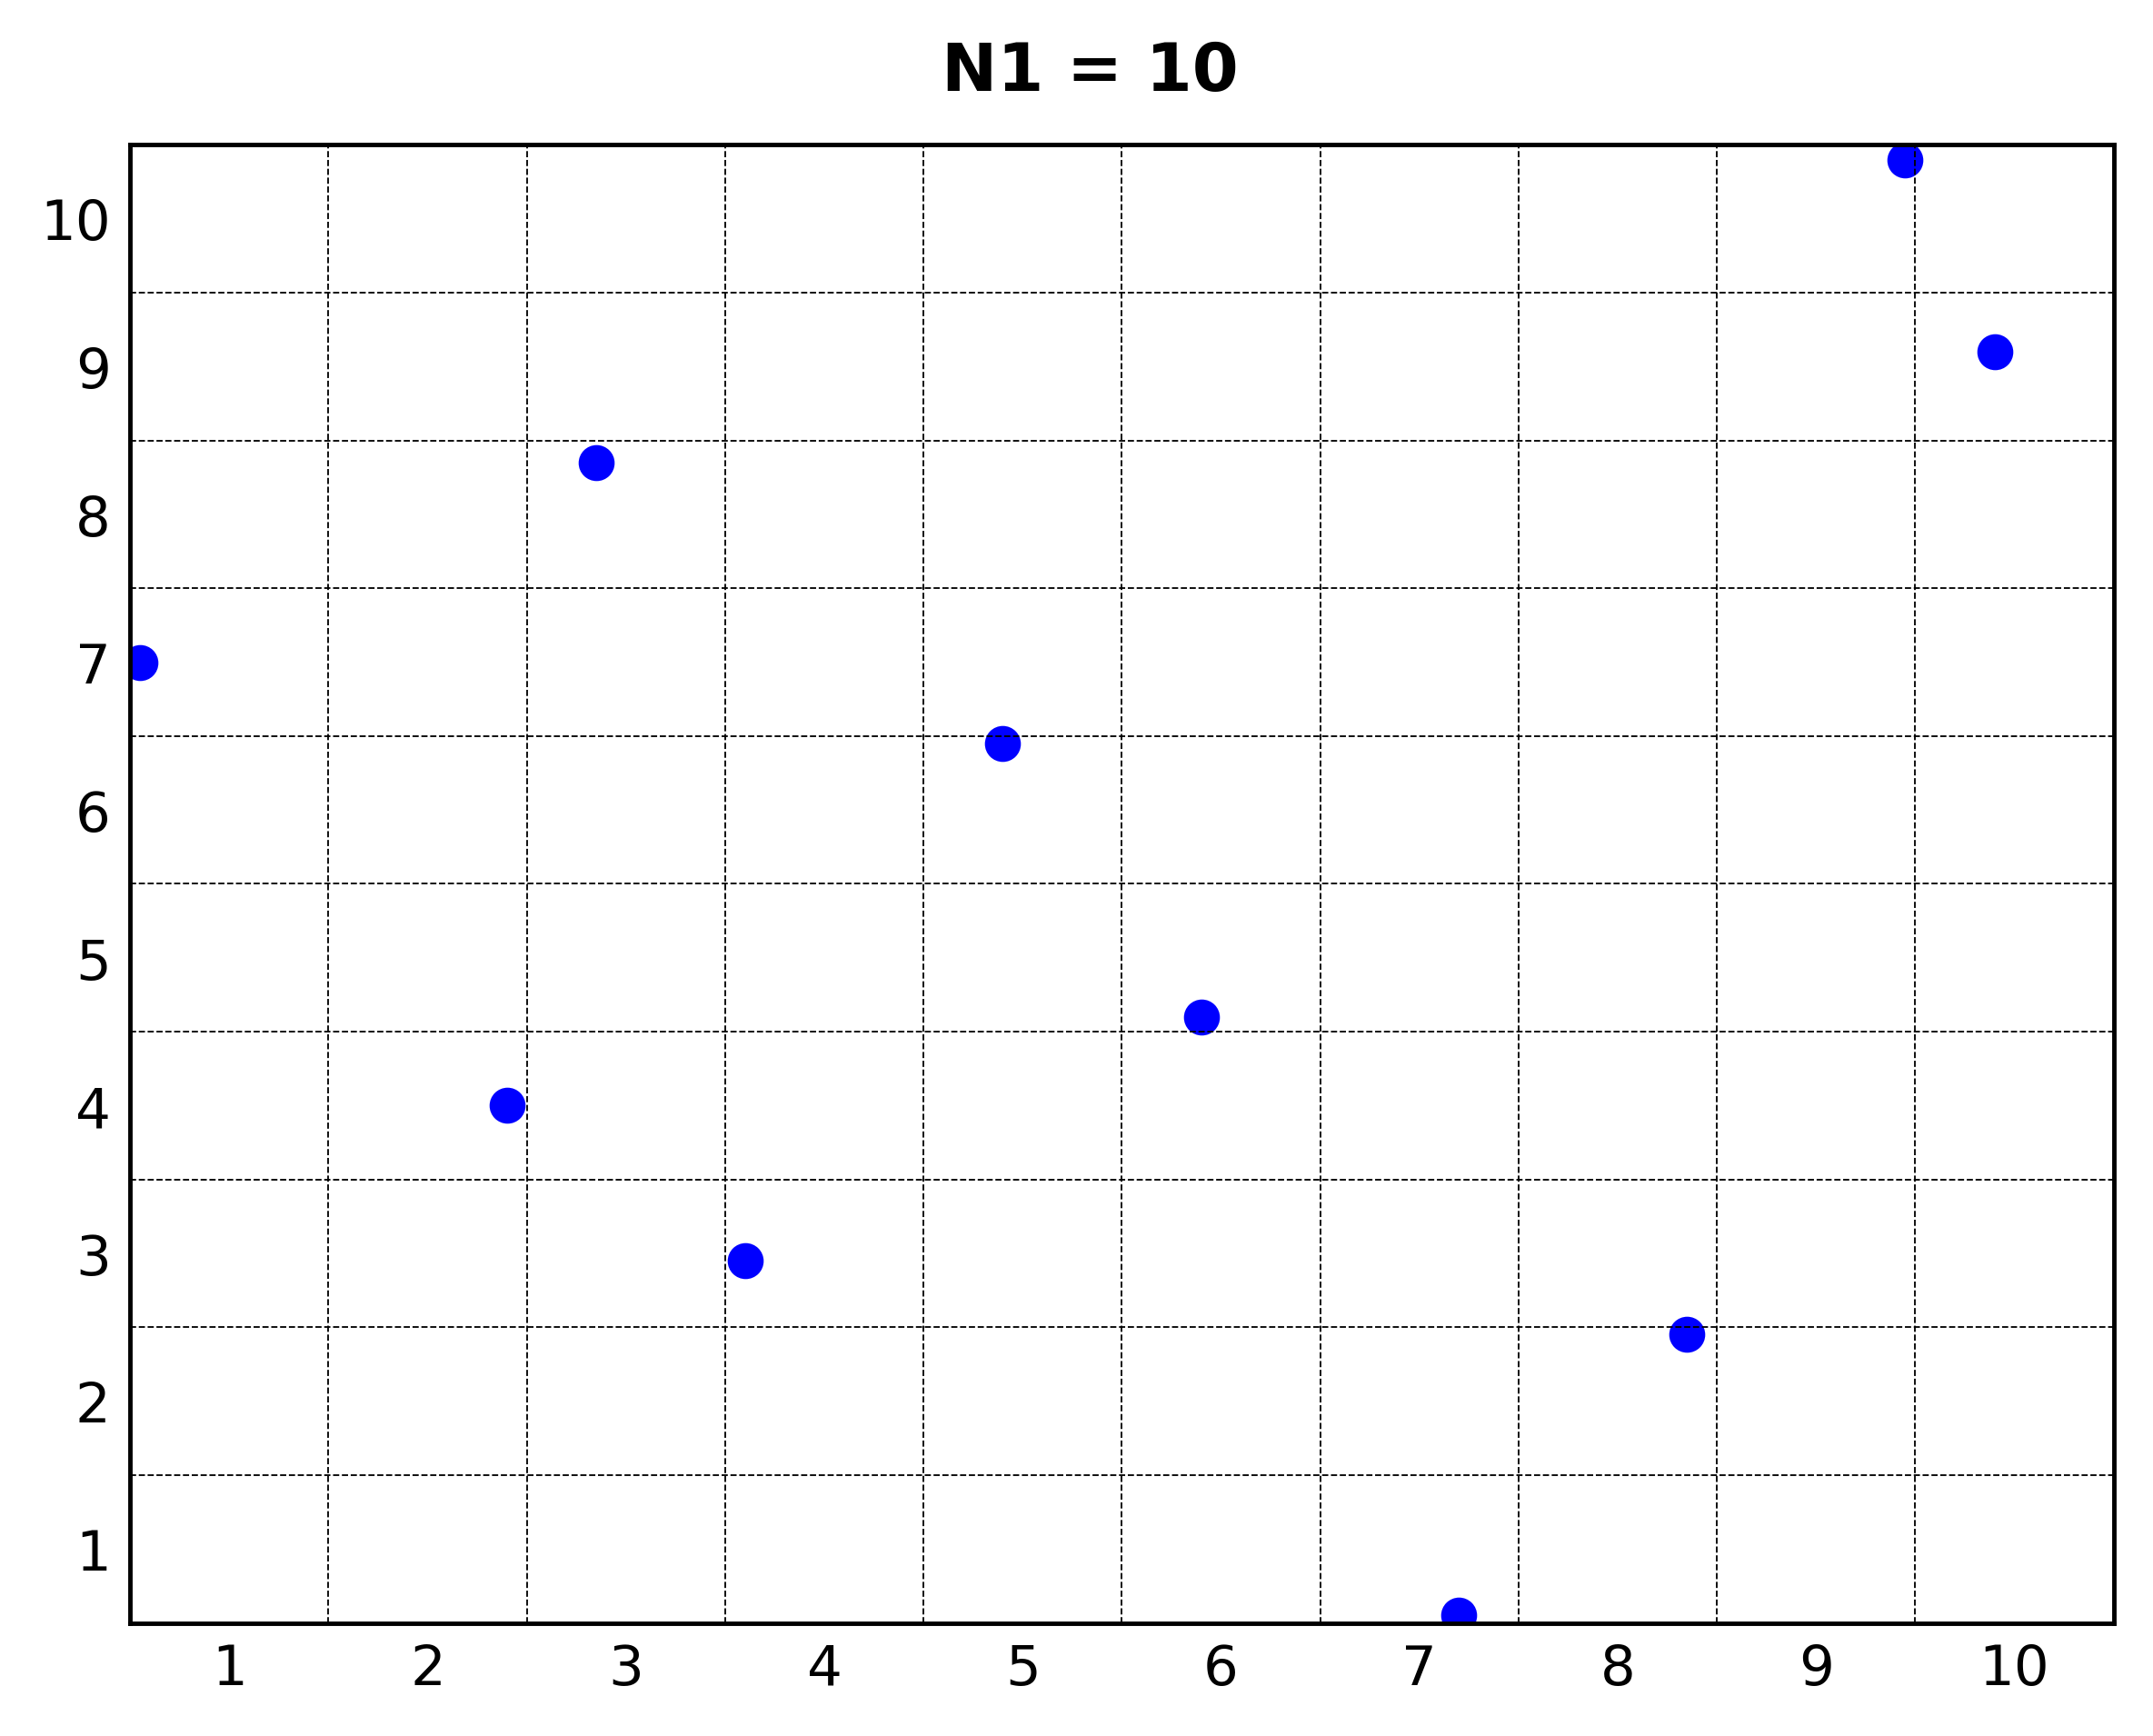
\includegraphics[width=\textwidth]{src/imgs/example_overlaps1.png}
        	\captionsetup{skip=0pt}
        	\midcaption{N = 10}
        	\label{fig:example_overlaps1}
        }
    \end{subfigure}
    %\hspace{0.05\textwidth}
    \begin{subfigure}[b]{0.49\textwidth}
        \centering
        \vtop{
        	\vspace{0pt}
        	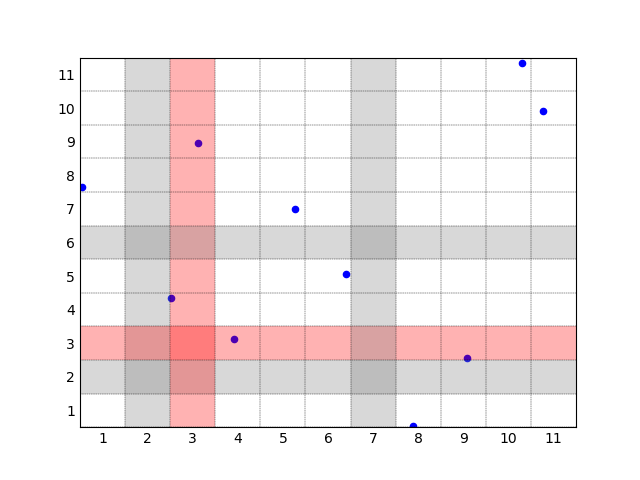
\includegraphics[width=\textwidth]{src/imgs/example_overlaps2.png}
        	\captionsetup{skip=0pt}
        	\caption{N = 11}
        	\label{fig:example_overlaps2}
        }
    \end{subfigure}
    
    \begin{subfigure}[b]{0.49\textwidth}
        \centering
        \vtop{
        	\vspace{0pt}
        	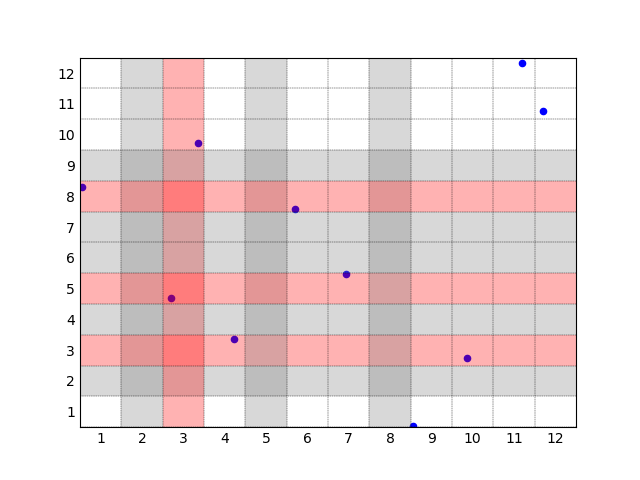
\includegraphics[width=\textwidth]{src/imgs/example_overlaps3.png}
        	\captionsetup{skip=0pt}
        	\midcaption{N = 12}
        	\label{fig:example_overlaps3}
        }
    \end{subfigure}
    %\hspace{0.01\textwidth}
    \begin{subfigure}[b]{0.49\textwidth}
        \centering
        \vtop{
        	\vspace{0pt}
        	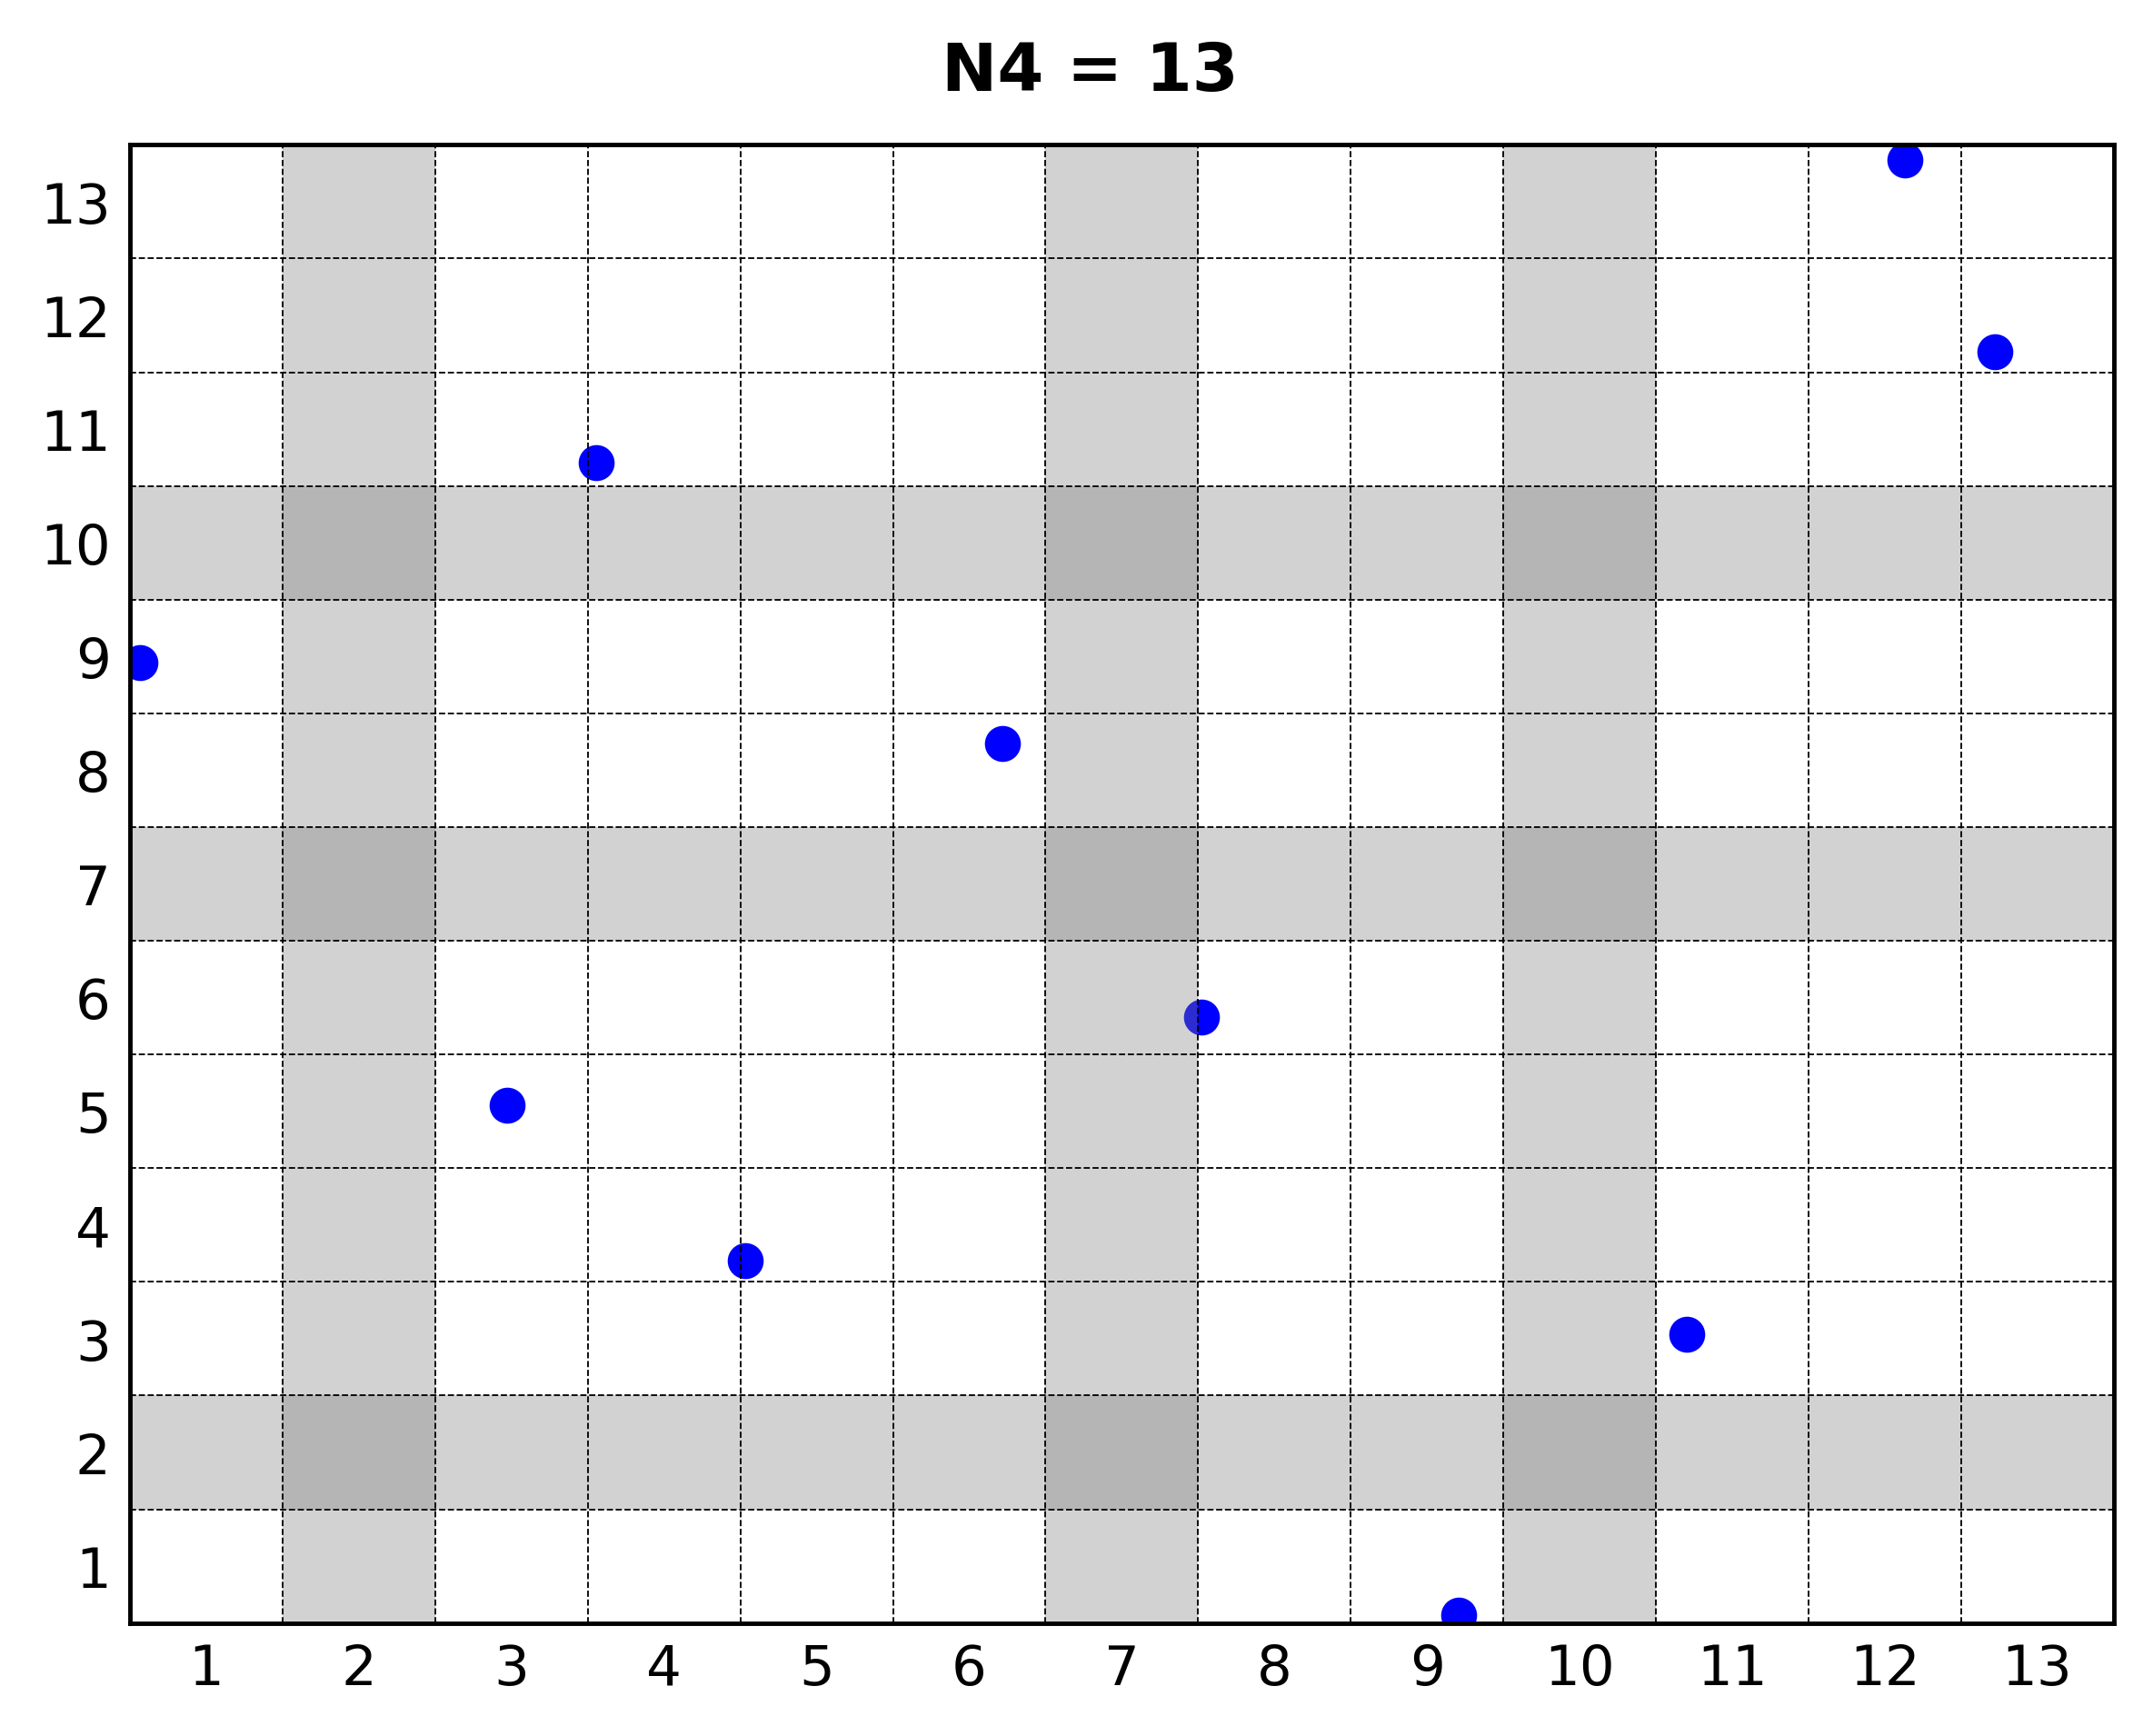
\includegraphics[width=\textwidth]{src/imgs/example_overlaps4.png}
        	\captionsetup{skip=0pt}
        	\midcaption{N = 13}
        	\label{fig:example_overlaps4}
        }
    \end{subfigure}
    
    \caption{To demonstrate the behavior of the grid, a $S$ LHS sample set is first created in a squared space ($P = 2$ dimensional hypercube) and projected over the grid as it grows one by one. Rows and columns marked in red indicate the locations of overlaps, while light grey-colored rows and columns are vacant. In (a) a fixed $N$ LHS samples are generated and displayed over a square of $N$ interval per axis; (b) shows the first step of the growing grid: two overlaps occur in interval horizontal \#3 and vertical \#3, two intervals per dimension are vacant one of which derives from the expansion vacancy and the other one is caused by the overlap; (c) samples displayed over $N + 2$ grid: on the vertical axis, 3 overlaps and 2 (from the expansion) + 3 (from the overlaps) vacancies; (d) the grown $N + 3$ grid have no collisions, then $S$ is a perfect expansion on $M = 3$ expansion magnitude [la sovrapposizione dei colori tra le evidenziature è fuorivante?]}
    \label{fig:example_overlaps}
\end{figure}

\subsection{Grade of an Expansion}
\label{subsec:expansion_grade}
A precise heuristic that expresses how near the current expansion is to a perfect expansion, given the desired expansion magnitude $M$ and the beginning state, is necessary for developing a new sample set. Since the metric in \meqref{eq:grade} is no longer sufficient, the variation \textit{expanded grade} has been offered.
The purpose of the \textit{expanded grade} is to convert the sample set $S$ of $N$ elements into a percentage index when the sample set is compared against a $P$-dimensional hypercube grid of $N+M$ intervals per axis - this is where it deviates from \meqref{eq:grade}. Here it follows:

\begin{equation}
\label{eq:expanded_grade}
gr(S, M) := \frac{\sum^P_{j=1}\sum^{N + M}_{q=1} min(\sum^N_{i=1}\indfunc{[\frac{q-1}{N + M}, \frac{q}{N + M})}(S_{ij}), 1)}{P \cdot (N + M)}
\end{equation}

Each $I$ interval contributes to \meqref{eq:expanded_grade} value with a share of:

\begin{equation}
\label{eq:single_contribute_interval}
share_I = 
\begin{cases}
\frac{1}{P \cdot (N+M)} \qquad \text{\textit{if any x $\in$ I}}\\
0 \qquad\qquad\;\;\; \text{\textit{otherwise}}
\end{cases}
\end{equation}

which makes \meqref{eq:expanded_grade} a discrete quantity that ranges from $\frac{1}{N+M}$, if every sample of a non-empty set lies in one single interval per axis, to 1, which represents the perfect LHS expansion and it's a multiple of \meqref{eq:single_contribute_interval}.

Considering the $N+M$ space grid of a perfect expansion from $S$ of $N$ samples over $M$ new intervals, given that in such a space would be covered by $N$ samples in $N$ distinct intervals per dimension by definition of LHS, a number $M$ of intervals per dimension is left empty. Then, the shares of the empty intervals are none, against the positive shares given by the $N$ others. From this statement, we can provide an upper limit for the expanded grade by starting from 1 - the maximum possible index of a perfect LHS sample set - minus the total weight lost during the growing of the grid, which corresponds to the total number of \textit{voids} times \meqref{eq:single_contribute_interval}. The total number of \textit{voids} is given by $M \cdot P$ because they are evenly spread across each dimension. So, $Z$ is a \textit{perfect expansion} of $S$ on $M$ new samples if and only if:

\begin{equation}
\label{eq:upper_limit_perfect_expansion}
gr_{max}(S, M) = 1 - \frac{M}{N+M}
\end{equation}


\subsection{The expansion process}
The expansion task was initially handed at the very beginning of  \cref{subsec:multistage_task} as a evolutionary process which augments the $S$ starting sample set to a next-stage state with increased number of elements $M$, placed as better as it can to maximize criteria. We do also said at \cref{subsec:expansion_grade} that an expansion may demote the non-collapsing property of the resultant expanded set $Z$, which can be measured with the metric \meqref{eq:expanded_grade}. 
In this section the authors propose how to place the new samples to achieve maximum "LHS-ness" over any $M$ expansion magnitude needed and introduce its potentialities for future researches - an interested reader should see \cref{sec:conclusions}.

In first place, the proposal is delivered by studying the basic case of a perfect expansion in \cref{subsubsec:perfect_expansion_case}, then extend to the general case with any non-perfect expansion outcome.

\subsubsection{State case - Perfect Expansion}
\label{subsubsec:perfect_expansion_case}
Referring to \cref{subsec:expansion_grade}, from an initial instanced sample set $S$ of $N$ elements, the experiments can be perfect expanded if and only if $S$ after the $M$-th step growing of the $P$ hypercube grid has max grade \meqref{eq:upper_limit_perfect_expansion}. Furthermore, \mfigref{fig:example_overlaps4}, which is a perfect expansion of $S$ with $M = 3$, well depicts the situation which the experimenters would expect to encounter before setting down the expansion set $E$. We notice the best candidate extent is likely the empty intervals (in light grey) because they do not interfere with other well-formed intervals. It's also imperative that the scattered new points don't stupidly overlap onto each other over the vacant space, hereby \textit{vacancies} or \textit{voids} for sake of simplicity.

First of all, it's necessary to trace each void's index. Here it comes into use again the (permuted) index matrix, previously used in \cref{subsec:how_to_lhs} to scatter the samples across the hyper parameter space. By the way, the matrix of voids $P \times M$ is composed by the row vectors: 

\begin{equation}
\label{eq:voids_matrix}
\textbf{V}_j = \bigg( z : \nexists\; x \in S_{ij} \; s.t. \; x \in \Big[\frac{z}{N+M}, \frac{z+1}{N+M}\Big) \bigg) \quad, \quad \forall j = 1...P
\end{equation}

which should be column-permuted along each row to prevent \mfigref{fig:diagonal_poor_design} diagonalized situation.
Then, the expansion set $E$ collects all the newly generated samples which are a distribution likewise \meqref{eq:rand_variable_Sij} but based using $V_{ji}$. 

In the end, the initial $S$ set is concatenated with expansion set $E$, originated from the voids of the $N+M$ growing grid, in a perfect expansion, that guarantees the fulfilling of the non-collapsing property (grade = 1). 

A perfect expansion is a intuitively rare event: no samples have to overlap with anyone else, which can be excluded if two sample projections are spaced more than $\frac{1}{N+M}$ apart (new size of the intervals). Furthermore, for any $M$ close to $N$, a \textit{critical span} exists across the right border of the i-th interval - namely \textit{i-th frontier} (see right after \meqref{eq:interval_index} for definition) - where two samples might be placed in, during the first stage of LHS sampling. An example of how can a couple of collapsing samples can occur is shown in \mfigref{fig:critical_span}. The critical span is identified by the new interval created across two old ones, which the first sample is in \mfigref{fig:critical_span2} has been generated in the critical area \textit{$\sim$2} intersected with \#1 original interval. On its hand, the second sample lies upon the intersection between \textit{$\sim$2} and \#2 original subspace.

\begin{figure}[h]
    \centering
    \begin{subfigure}[b]{0.45\textwidth}
        \centering
        \vtop{
        	\vspace{0pt}
        	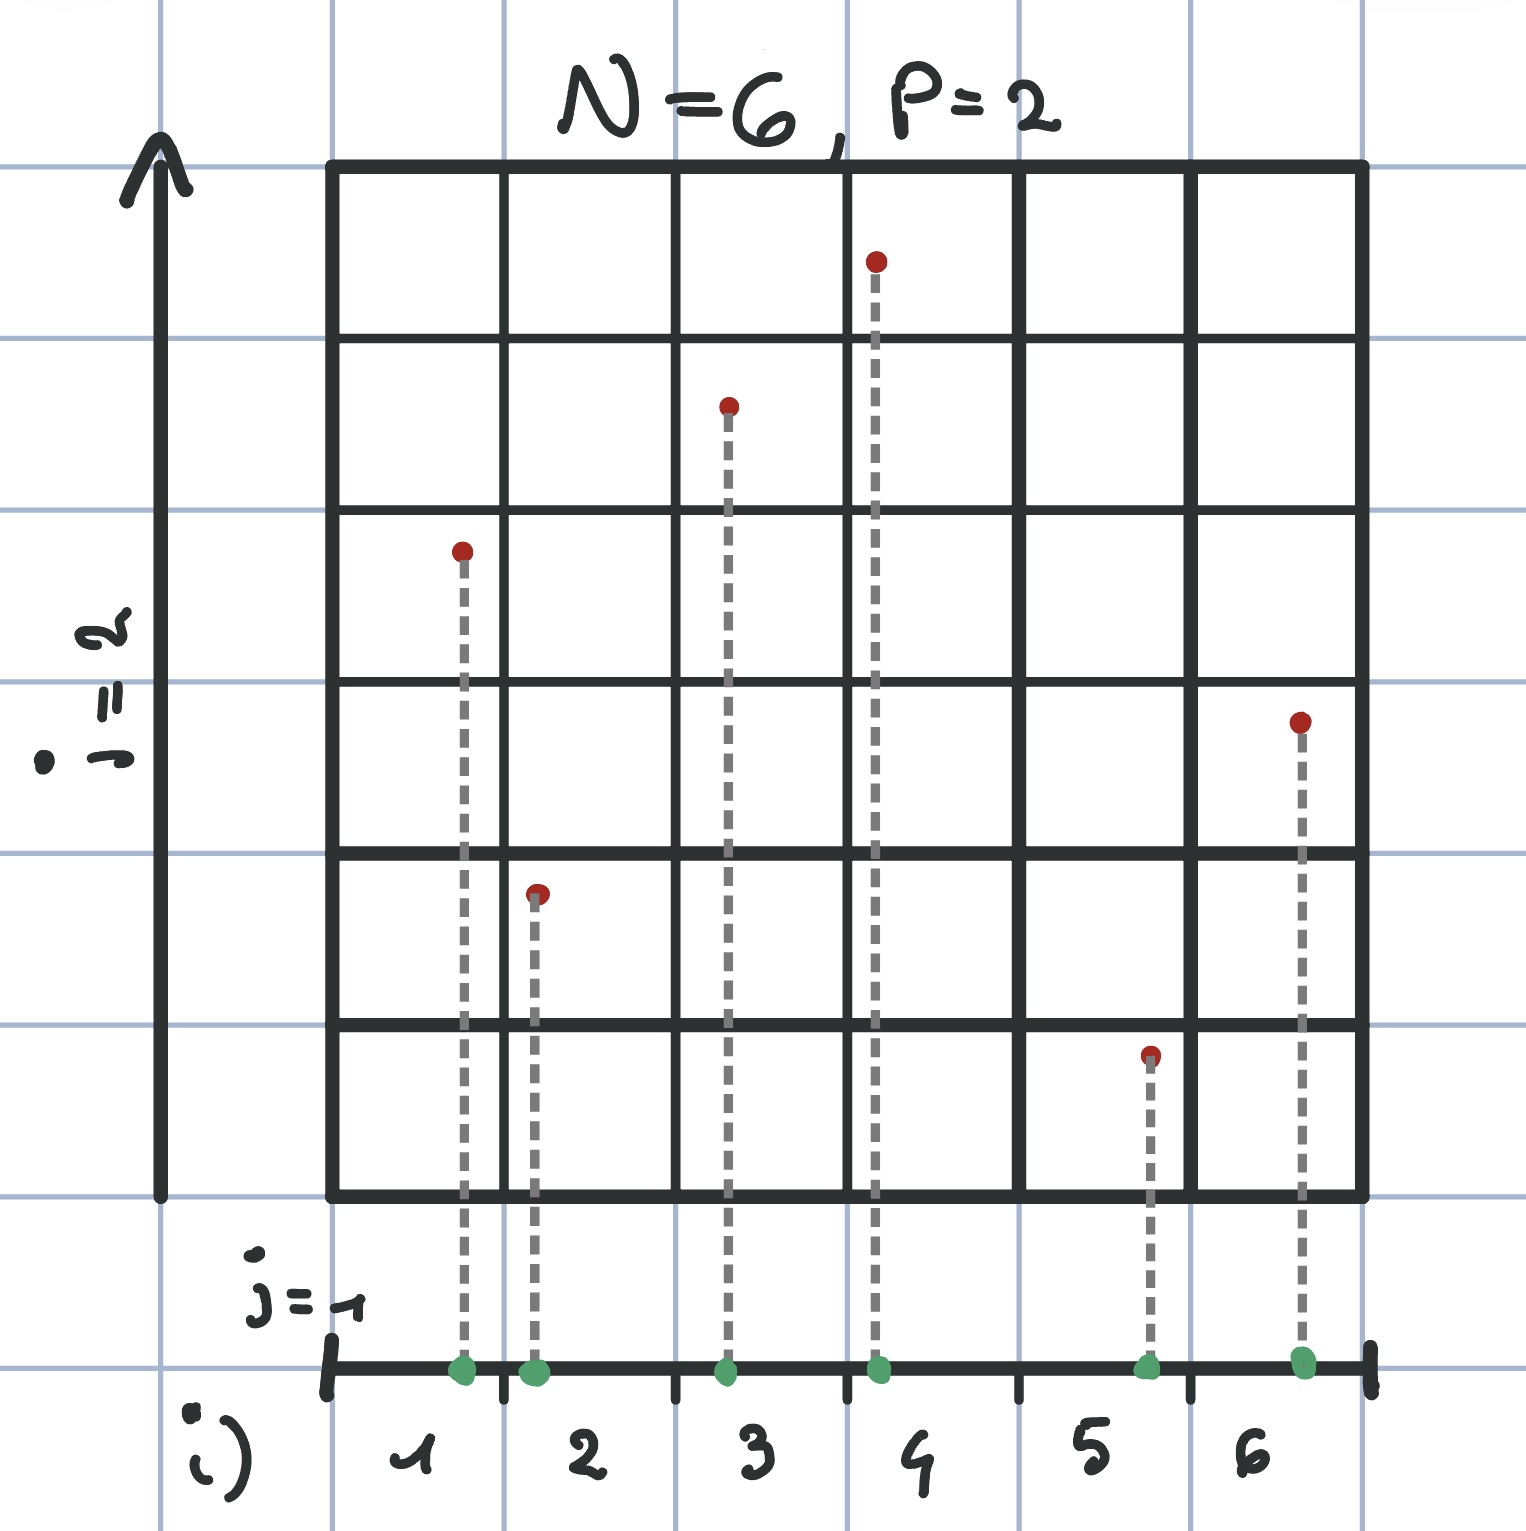
\includegraphics[width=\textwidth]{src/imgs/critical_span_init.jpg}
        	\caption{An LHS of $N = 6$ samples expanded for $M = 2$. on the horizontal axis are projected the horizontal component of all samples. [SKETCH - ne farò in digitale di migliori]}
        	\label{fig:critical_span1}
        }
    \end{subfigure}
    \hspace{0.05\textwidth}
    \begin{subfigure}[b]{0.45\textwidth}
        \centering
        \vtop{
        	\vspace{0pt}
        	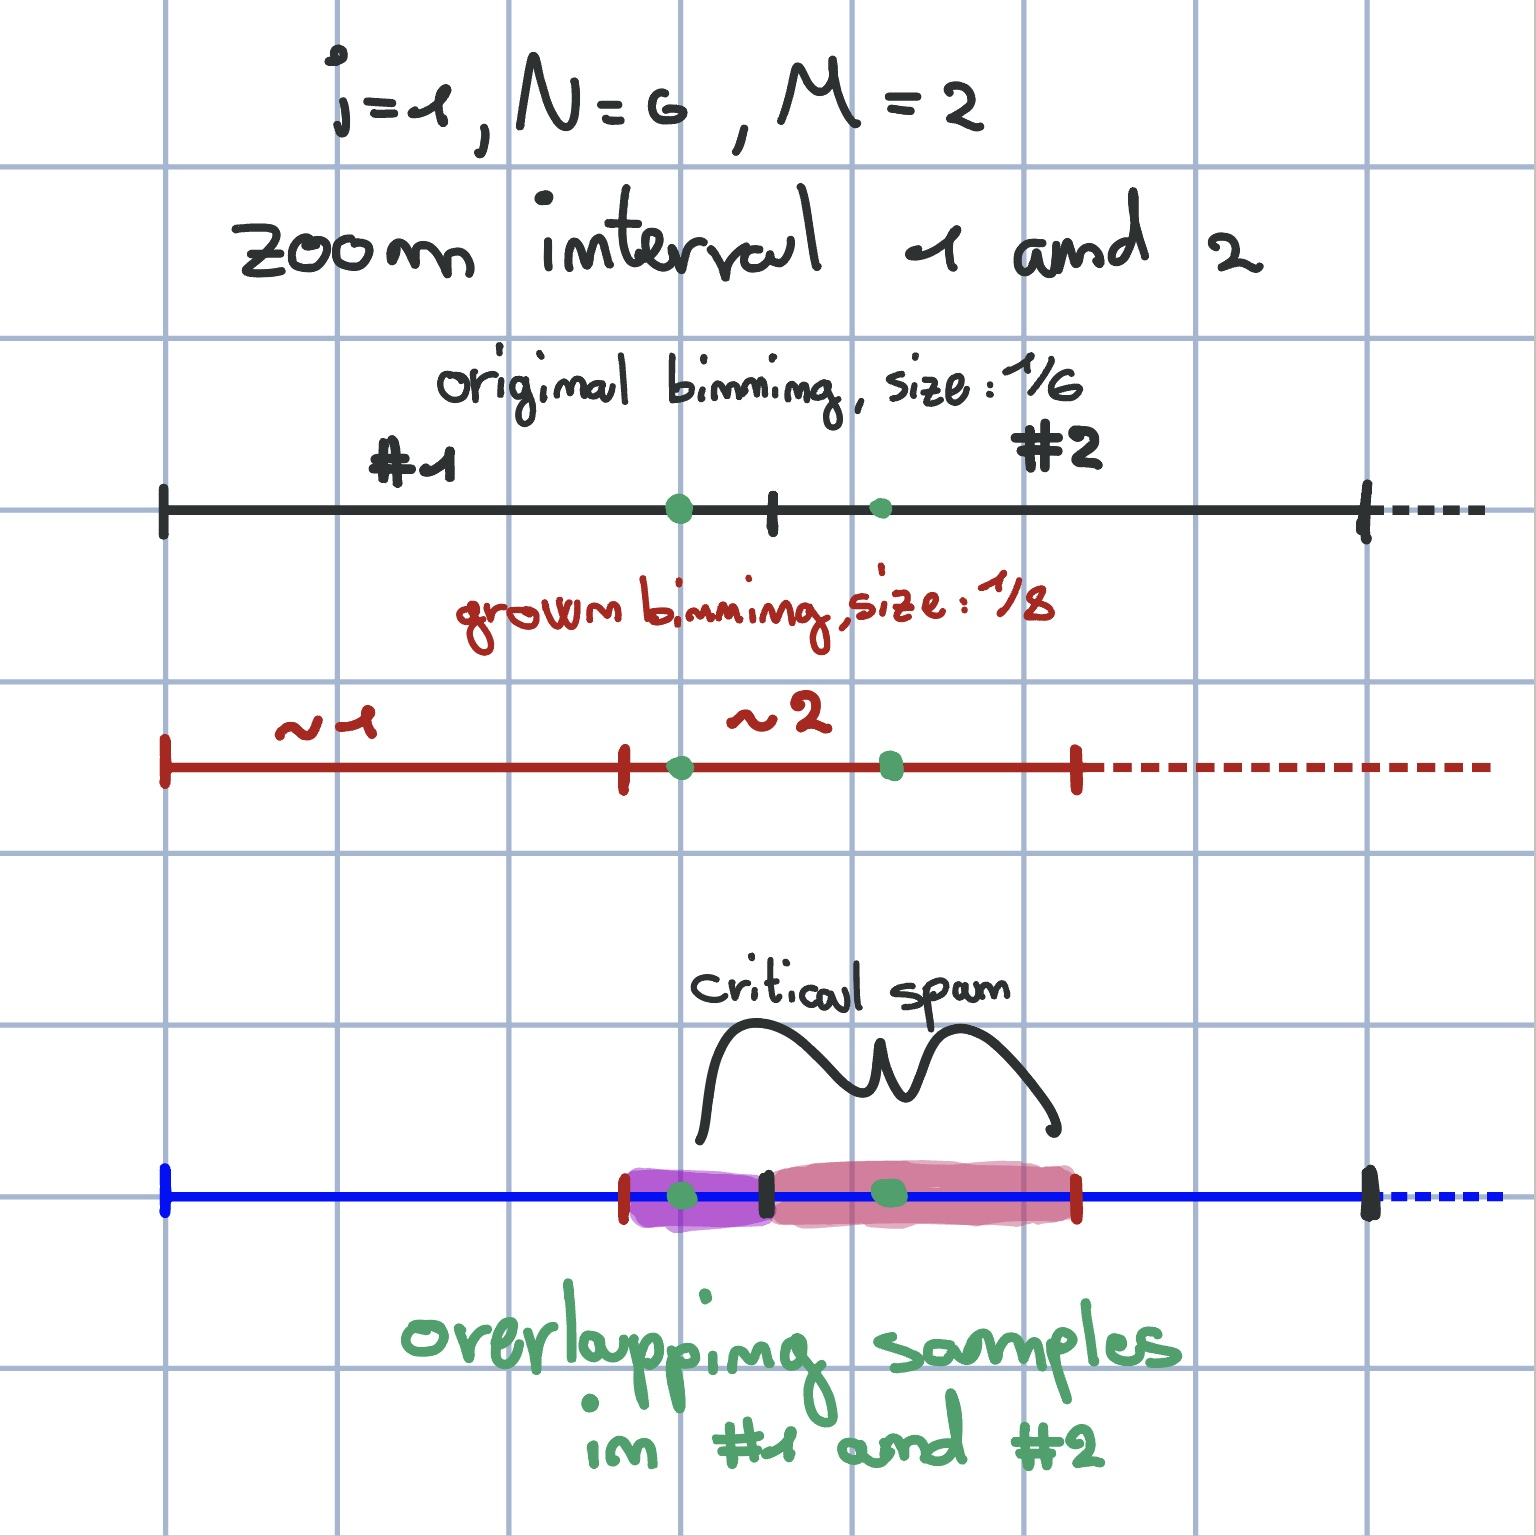
\includegraphics[width=\textwidth]{src/imgs/critical_span_zoom.jpg}
        	\caption{Zooming in \#1 and \#2 interval, it's show how both shares a critical area (on the bottom) whereof each one may have been distributed in it. [SKETCH - ne farò in digitale di migliori]}
        	\label{fig:critical_span2}
        }
    \end{subfigure}
    \midcaption{ }
    \label{fig:critical_span}
\end{figure}

\subsubsection{State case - General Expansion}
\label{subsubsec:general_expansion_case}
Because of \meqref{eq:expanded_grade} complexity, it's an harsh to predict which samples are going to overlap after the re-binning of the hypercube and/or which $M$ will produce a perfect expansion - and so a perfect expanded LHS, see \cref{subsubsec:perfect_expansion_case}.
During the upscale of $S$ sample set from $N$ to $N+M$ number of elements, it comes along with an $O$ number of overlaps.
In \cref{subsec:expansion_grade} was noted the relation between the number of vacancies row vector $\textbf{V}_j$, the magnitude of the expansion $M$ and the amount of collisions in the j-th dimension. Specifically:
\begin{equation}
\label{eq:vjojm}	% nome norvegese di alto rango
\parallel \textbf{V}_j \parallel = O_j + M
\end{equation}
whereof the overlaps count equals to zero, the expansion has been perfect (see \cref{subsec:multistage_task}). In a general case of expansion, the overlaps amount is most likely not equal to zero for some j-th dimensions.

The case study implies that the creation of $E$ expansion set is not trivial anymore because of the irregularity of the vacancies set. By stressing what \meqref{eq:vjojm} states, $V$ would probably be no matrix at all. 
The number of $\textbf{V}_j$ interval indexes would likely be more than $M$ sample's projections to commit. The expansion algorithm has to pick up a reasonable subset of $M$ void entries, and thus to discard an amount of intervals equal to the number of overlaps $O_j$. Therefore, given the sub-hyperspace settled by the joined selected voids, in order to plot an $M$ amount of new samples, it will pick up an $P \times M$ submatrix (that mimics \meqref{eq:voids_matrix}) of $V$ set. The submatrix should be handled being aware that it would effect the samples layout which may better improve another coherent criteria chosen (such as low-discrepancy or Maximin space-filling).\\
The selection process of vacancies from an irregular $V$ voids set is described by a function $\sigma: N \times P, \; M \rightarrow P \times M$, namely \textit{perfectify} or \textit{vacancy reduction} for the matter of giving names to anything. \\ 
In this section, $\sigma$ reduce function trivially picks up $M$ intervals randomly per dimension and build up a permuted \meqref{eq:voids_matrix} vacancies matrix, which will be plugged into \meqref{eq:Sij_def} to produce an $E$ expansion set. 

In other words, $\sigma$ criterion extracts from each j-th axis vacancies set $\textbf{V}_j$ a fixed $M$ number of elements which are going to compose the sub-hyperspace where $M$ samples will be placed in, using at least the non-collapsing property. The reduce function $\sigma$ discards $O_j$ number of intervals (\meqref{eq:vjojm}), then creating an amount of voids of the same quantity. Hence, the number of overlaps $O_j$ determines the number of void intervals after the expansion is consumed.

In this paper, the term \textit{quasi-LHS} refers to a non full-graded (grade equals to 1) n-th stage of expansion descended from a proper LHS.

\subsubsection{The eLHS algorithm}
\label{subsubsec:algorithm}
The LHS expansion algorithm, namely \textit{eLHS}, push a starting Latin Hypercube $S$ to the next stage $Z = eLHS(S, M)$ which best maximize (maintain) the non-collapsing property, along with other eventual criterions.

\begin{enumerate}
\item Instance a $V$ vacancies set of $P$ tuples - which may have different lengths (\meqref{eq:voids_matrix}) because every dimension has an arbitrary number of voids (\meqref{eq:vjojm}). The list of all indexes of the $N+M$ grid is filtered accordingly with \meqref{eq:voids_matrix}. \\ 
Visually, the algorithm re-bins the original $S$ grid (see \mfigref{fig:algo2} and \mfigref{fig:algo3}) to archive $N+M$ subdivisions. By plotting it against $S$, the reader can visualize where samples collide (overlap) and where there are none (void).

\item Reduce $V$ vancancies set to a suitable indexes matrix $V^\prime \in Matrix(P, M)$ by extracting from each $\textbf{V}_j$ tuple $M$ elements - which are going to compose the expansion binning grid - using $\sigma$ reduction criteria (see \cref{subsubsec:perfect_expansion_case}). If there are no overlaps (meaning $S$ has maximum expanded grade \meqref{eq:upper_limit_perfect_expansion}) then $V$ is implicitly equal to matrix $V^\prime$, so no reduction criterion is required to be applied.

\item Generate new points over the sub-hyperspace outlined by the permuted $V^\prime$ indexes matrix. Currently, Scipy hasn't implement instancing of a LHS over a discontinuous space yet.\\ 
To archive that, the algorithm sequentially draws $M$ samples from an optimal sample pool which have been determined by the others criterion applied (such as maximin space-filling, see \cref{subsec:lhs_properties}) where every samples are placed according with $V^\prime$
\end{enumerate}


%\begin{algorithm}
%\caption{eLHS}
%	\begin{algorithmic}[1]
%		\Require $S$: matrix $N \times P$
%		\Require $M$: int
%		\Ensure matrix $M \times P$
%		\Procedure{eLHS}{$S, M$}
%			\State $V \gets array[P]$
%			\State $A \gets array[P]$
%			\For{$i = 1 \text{to} i = P$ and $j = 1 \text{to} j = N$}
%        		\State $A_{ij} \gets (i-1)$
%	   		\EndFor
%	   	\EndProcedure
%		
		
%	\end{algorithmic}
%\end{algorithm}

\begin{figure}[h]
    \centering
    \begin{subfigure}[b]{0.45\textwidth}
        \centering
        \vtop{
        	\vspace{0pt}
        	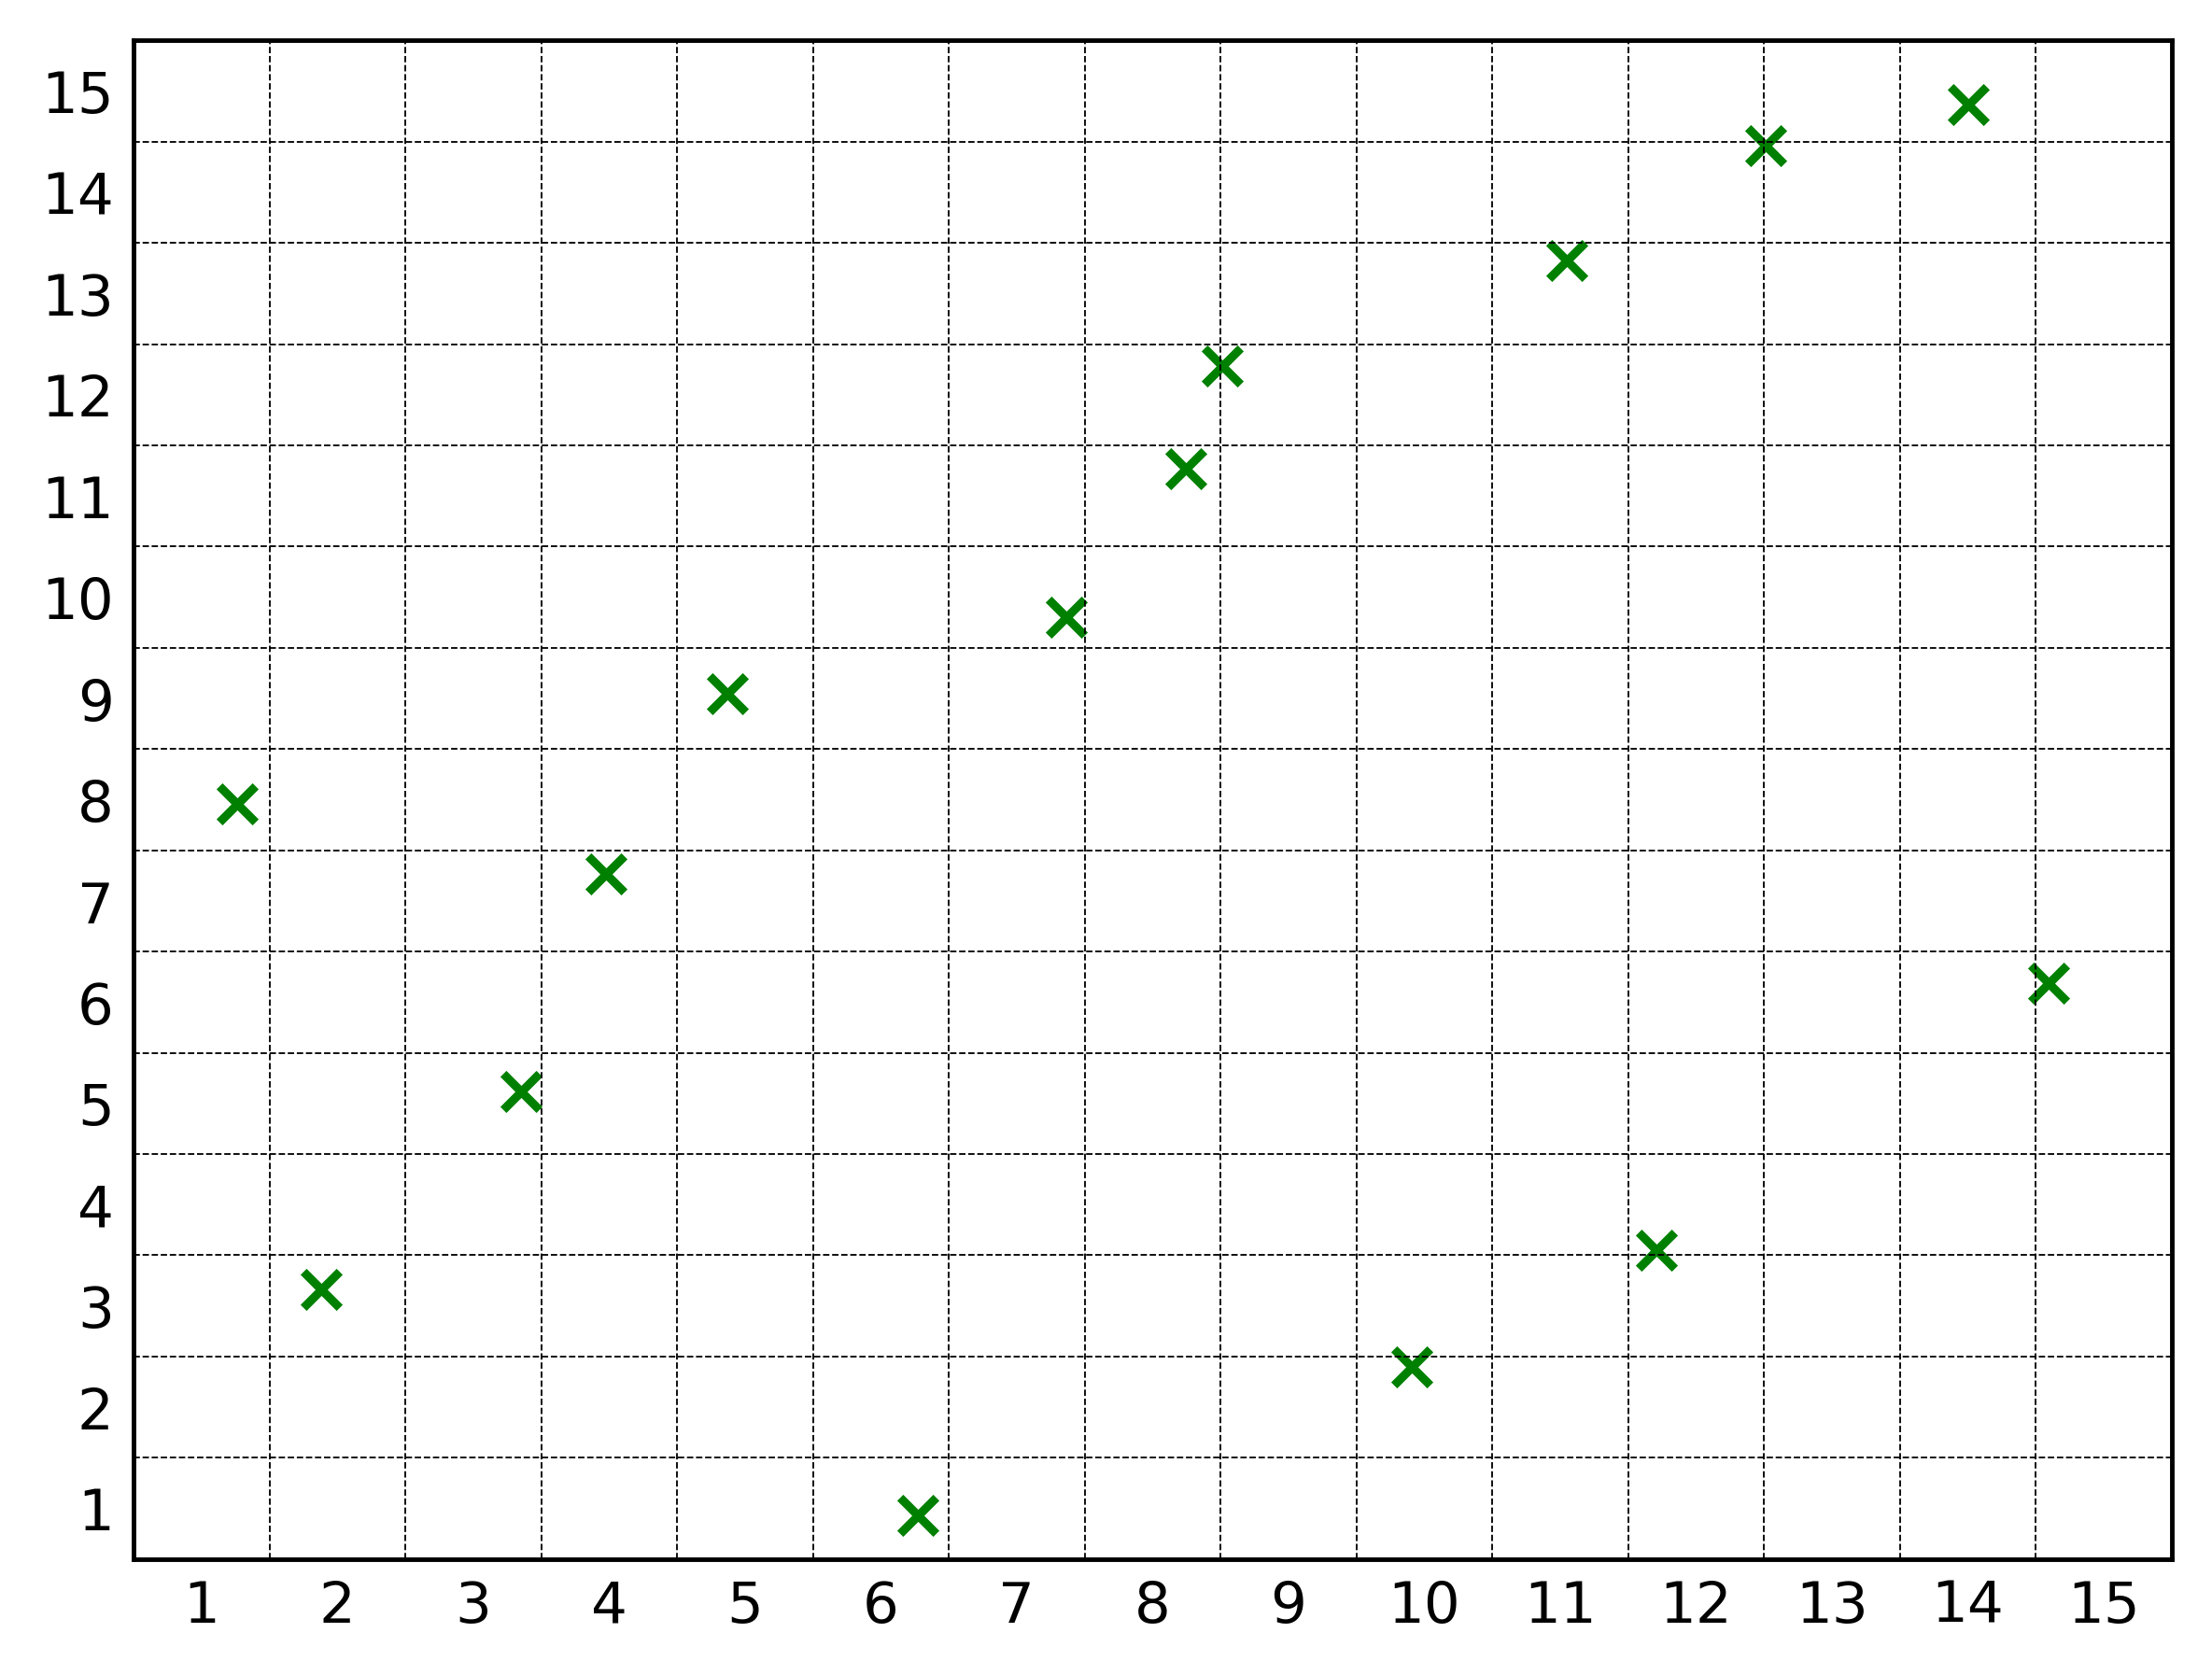
\includegraphics[width=\textwidth]{src/imgs/algo1.png}
        	\captionsetup{skip=0pt}
        	\caption{First-stage LHS of $N = 15$ samples in $P = 2$ generated with scipy's qmc library.}
        	\label{fig:algo1}
        }
    \end{subfigure}
    \hspace{0.05\textwidth}
    \begin{subfigure}[b]{0.45\textwidth}
        \centering
        \vtop{
        	\vspace{0pt}
        	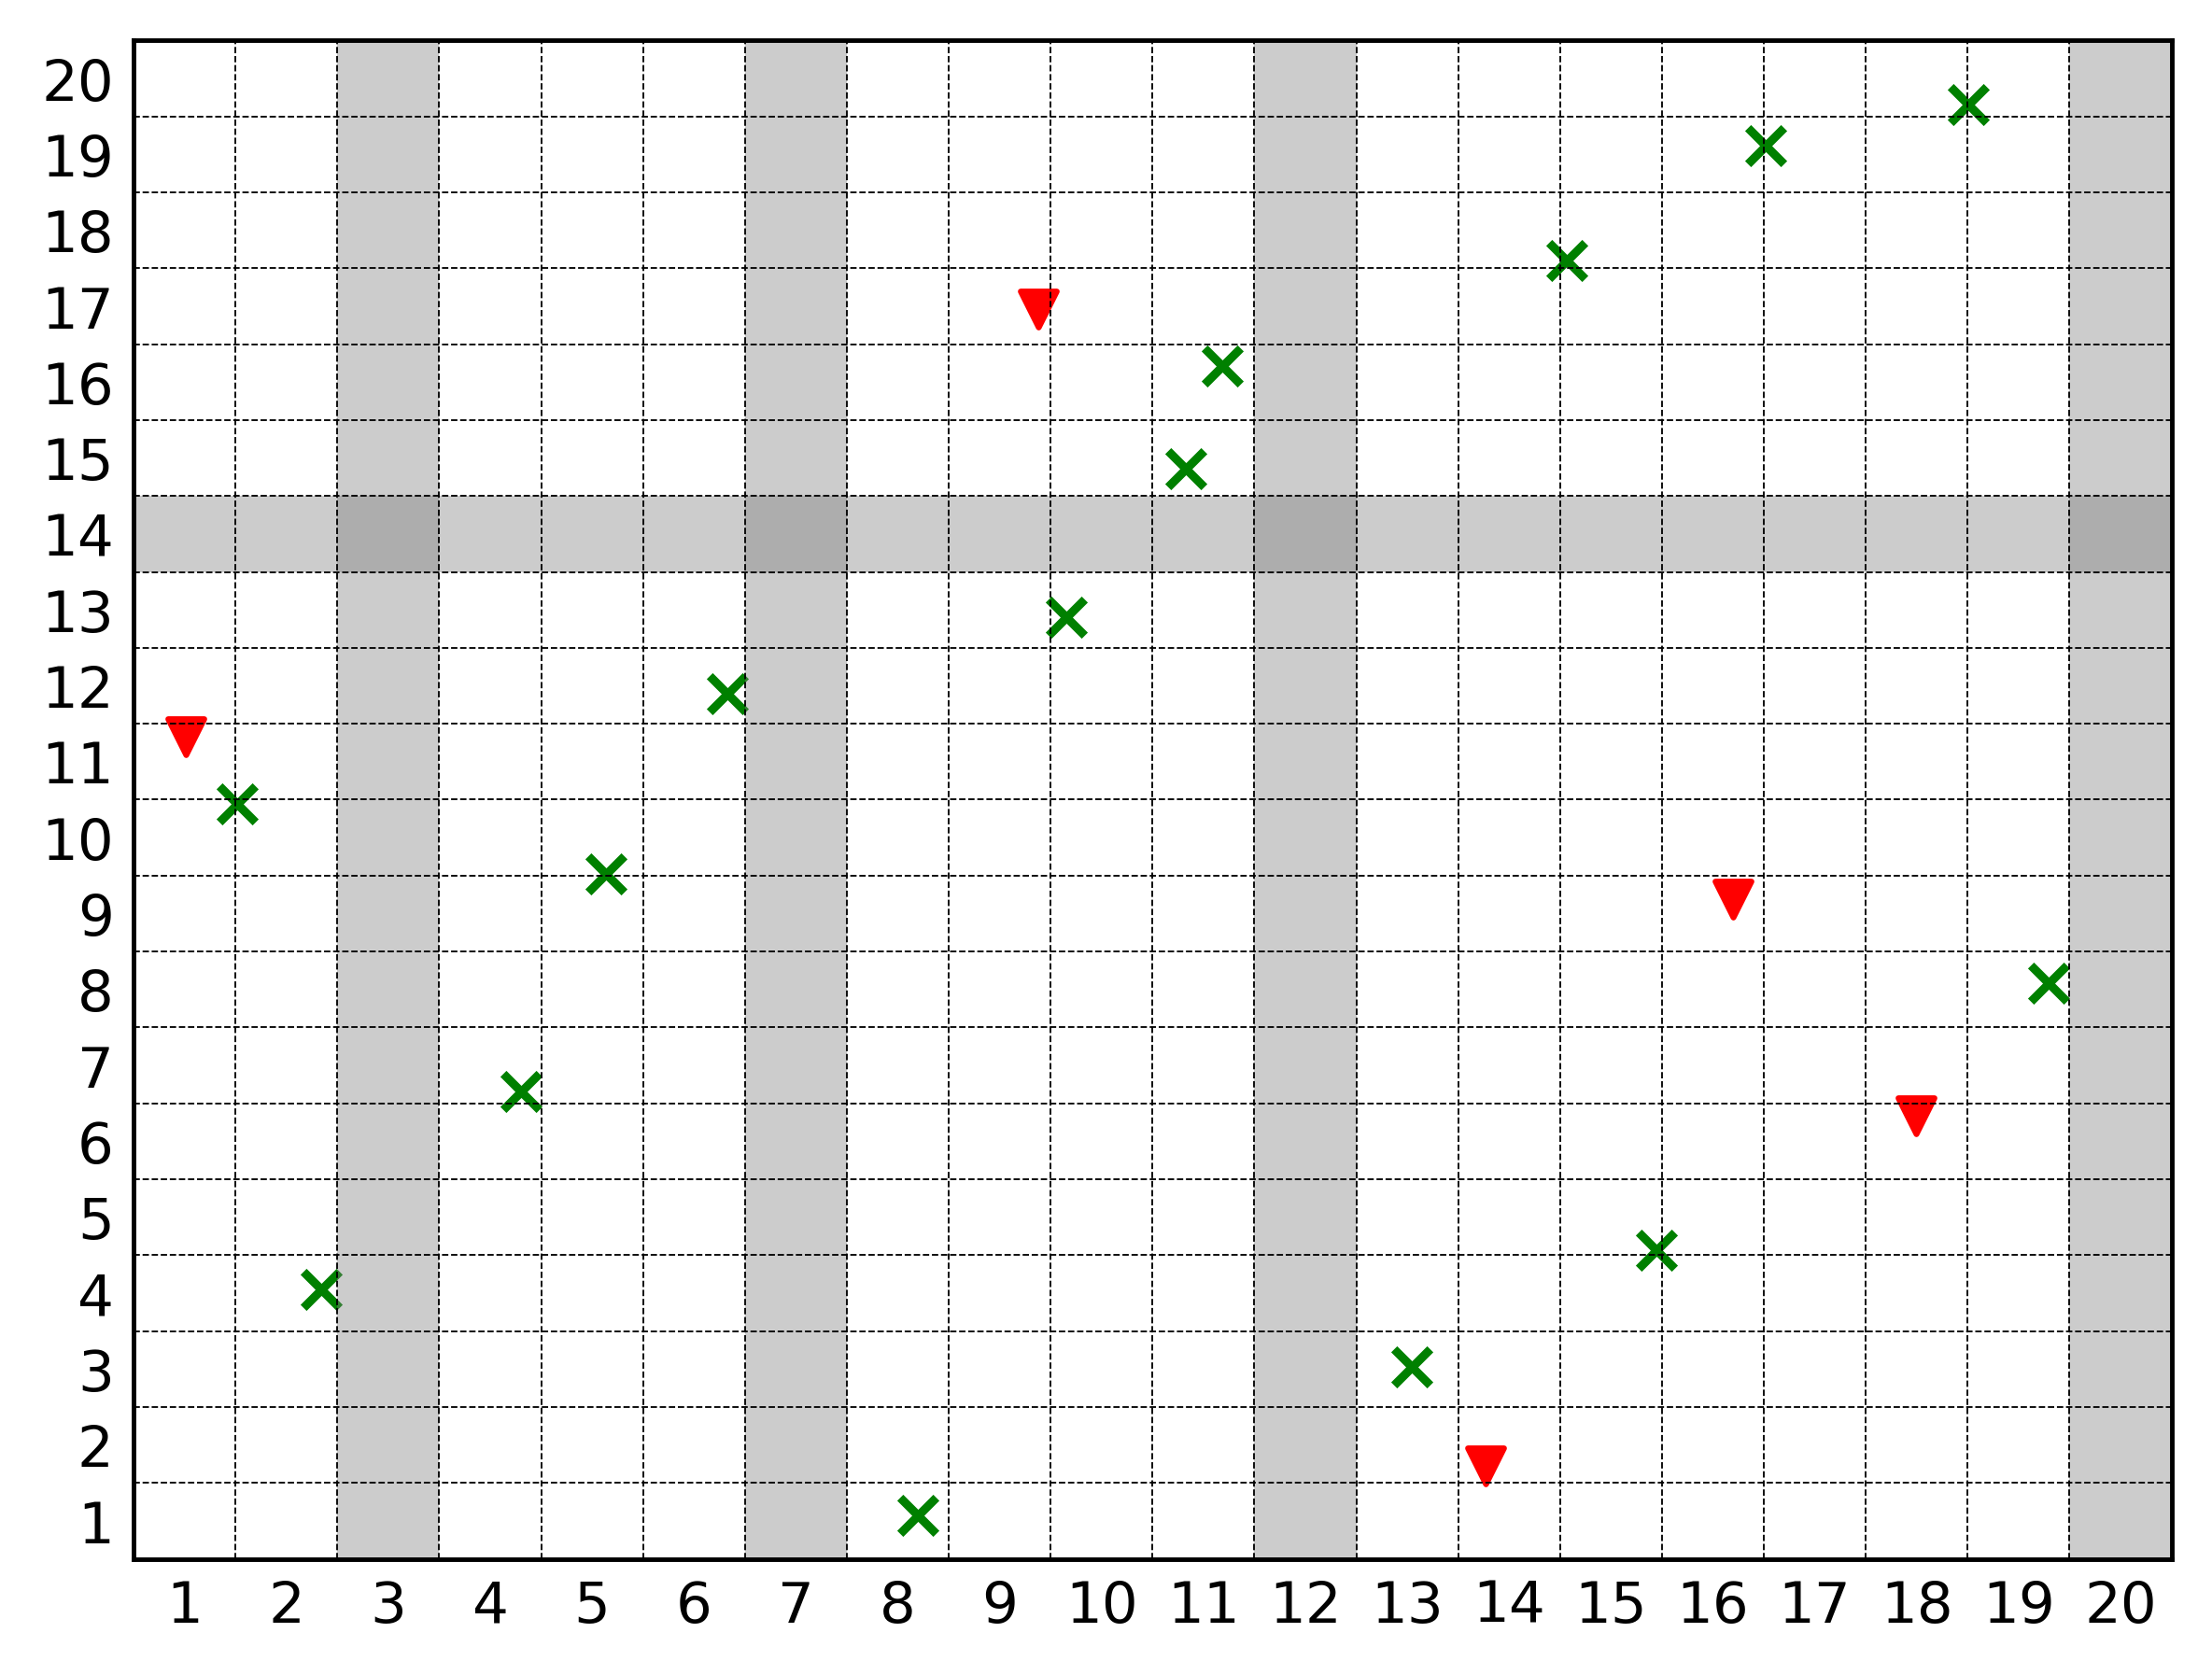
\includegraphics[width=\textwidth]{src/imgs/algo4.png}
        	\captionsetup{skip=0pt}
        	\caption{Expansion of (a)'s LHS with \cref{subsubsec:algorithm} eLHS algorithm given $M = 5$ new samples. Note that the light grey marked intervals are empty and, according to \cref{subsubsec:general_expansion_case}, they are related with the overlaps distribution in (c)}
        	\label{fig:algo2}
        }
    \end{subfigure}
    \captionsetup{justification=centering}
    \caption*{Above is shown a two-staged quasi-LHS. (a) is the first original LHS and (b) is next stage expansion of it.}
    
    \begin{subfigure}[b]{0.45\textwidth}
        \centering
        \vtop{
        	\vspace{0pt}
        	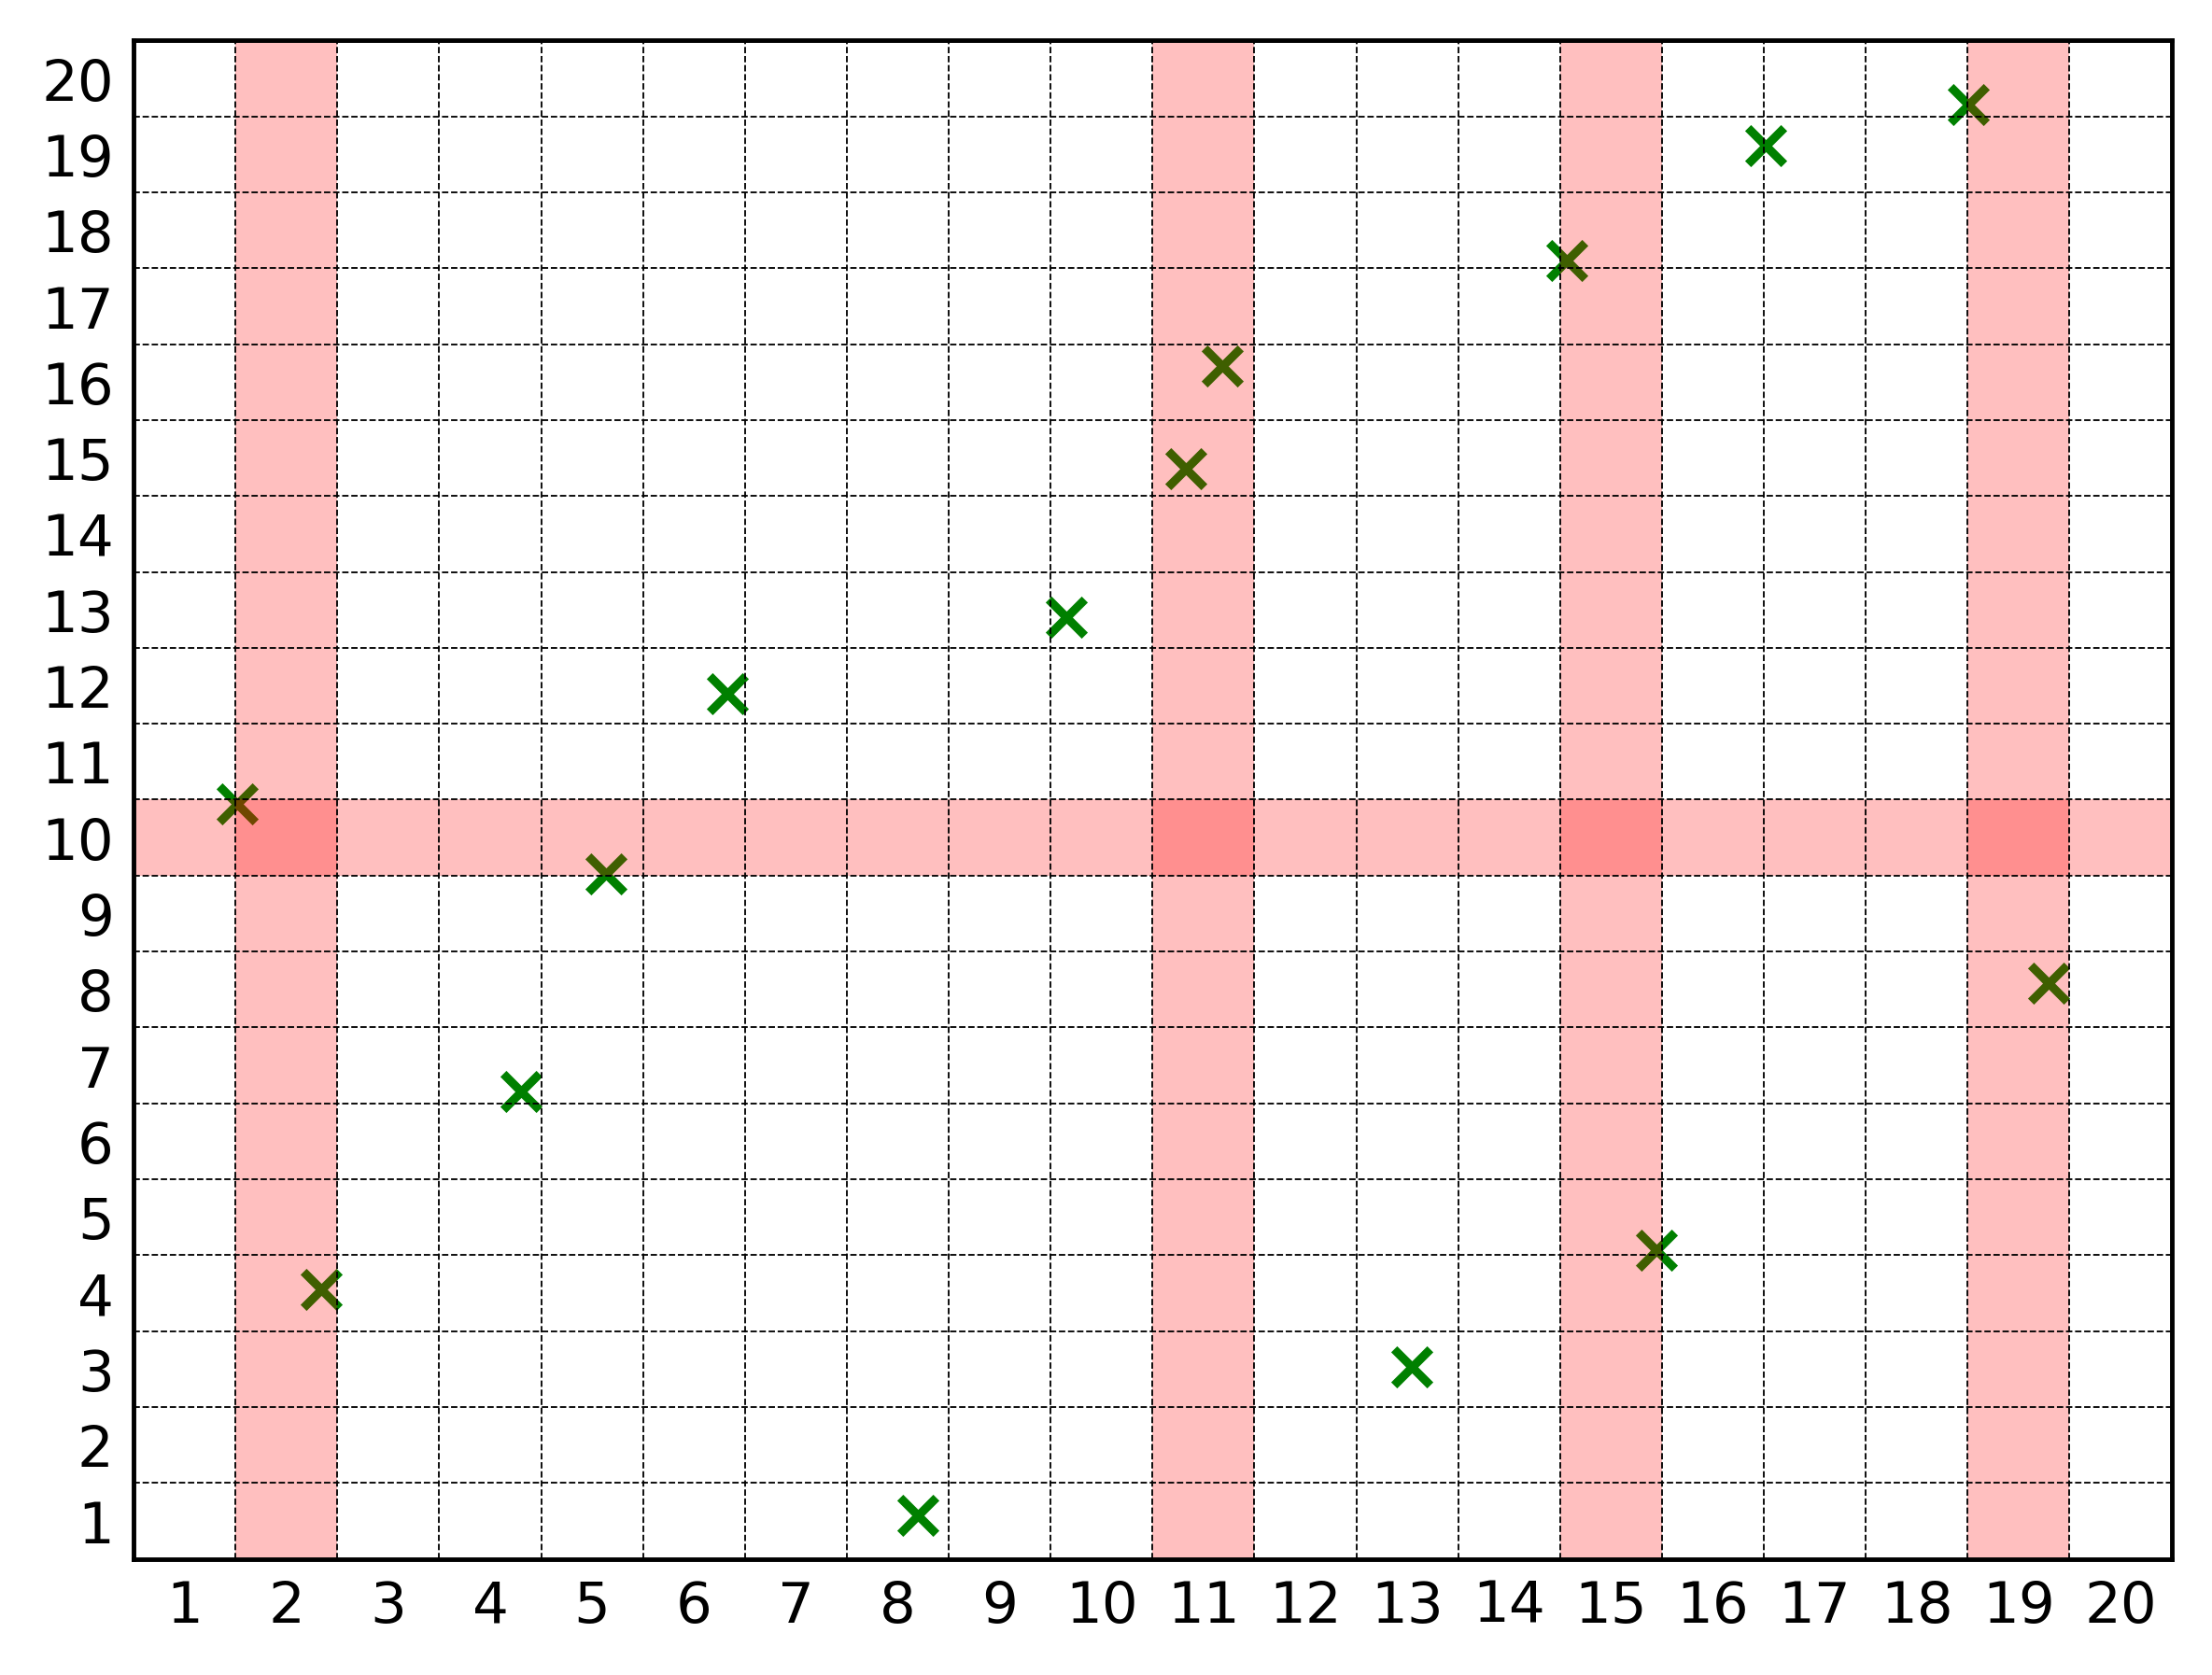
\includegraphics[width=\textwidth]{src/imgs/algo2.png}
        	\captionsetup{skip=0pt}
        	\caption{Red intervals have two sample's projections in it and break the non-collapsing property.}
        	\label{fig:algo3}
        }
    \end{subfigure}
    \hspace{0.05\textwidth}
    \begin{subfigure}[b]{0.45\textwidth}
        \centering
        \vtop{
        	\vspace{0pt}
        	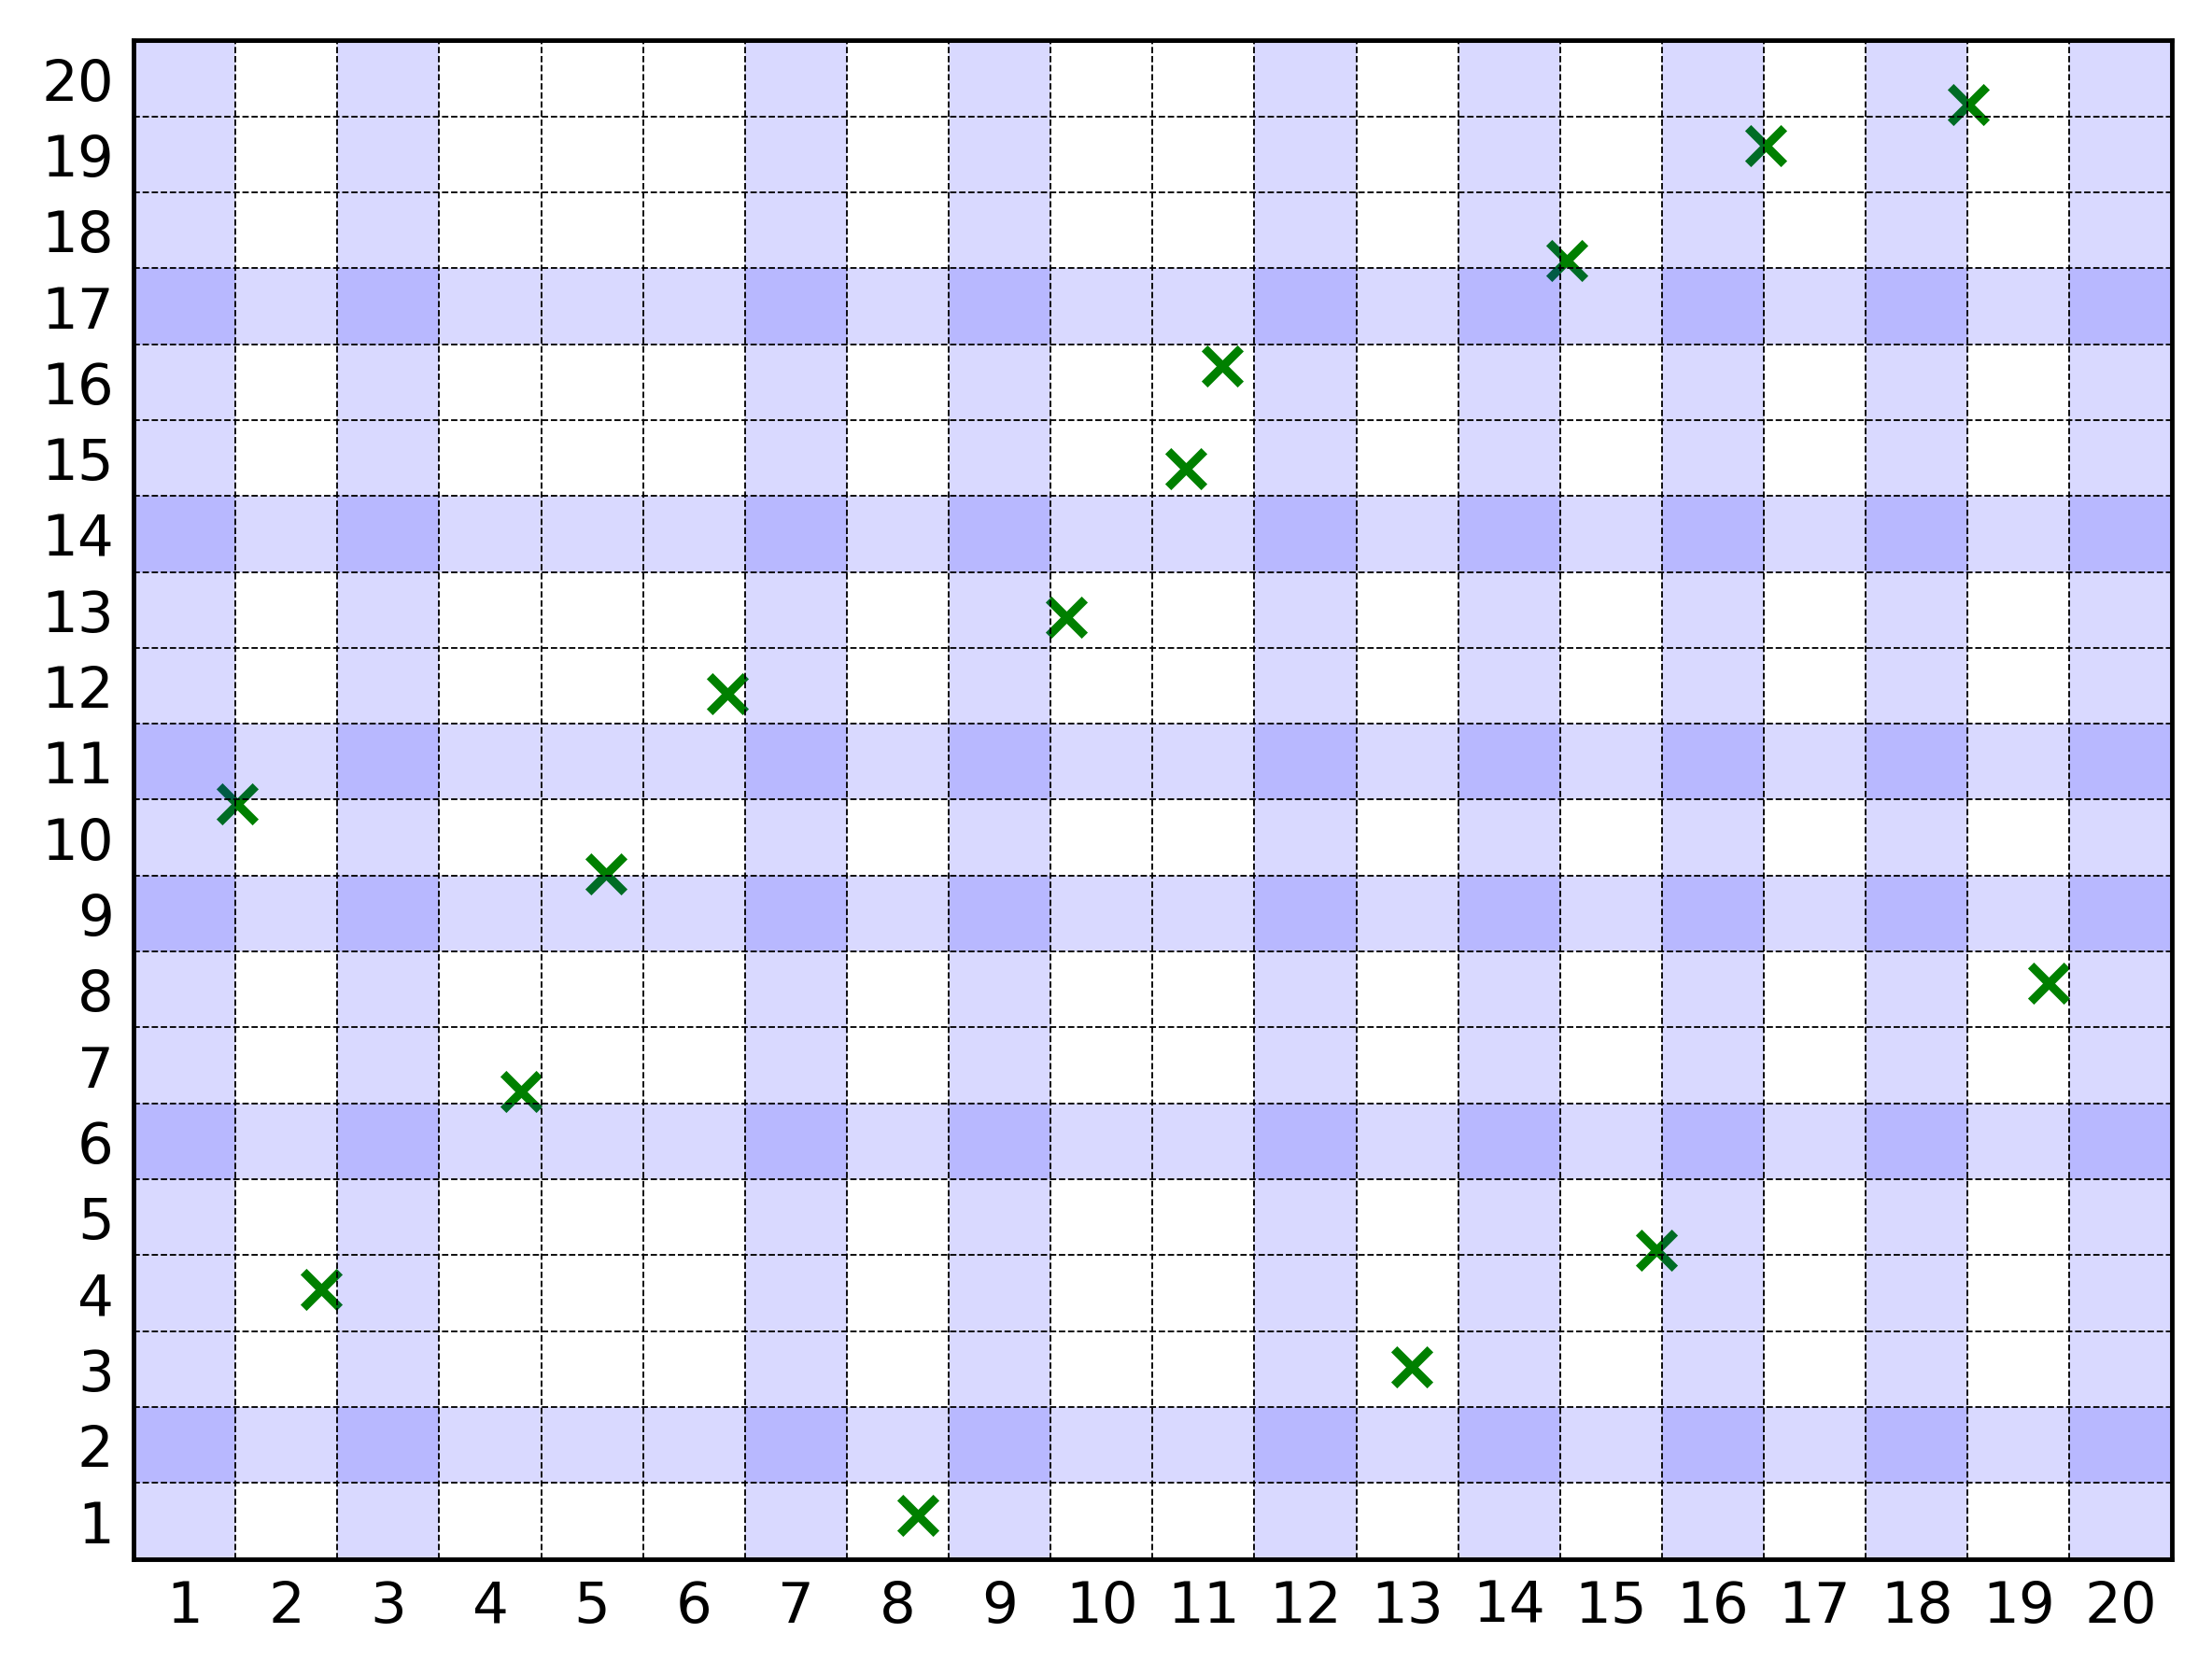
\includegraphics[width=\textwidth]{src/imgs/algo3.png}
        	\captionsetup{skip=0pt}
        	\caption{Blue intervals are empty. They represents the best candidate spots to place new LHS samples. Every interval all together has been referred as the sub-hyperspace of vacancies. }
        	\label{fig:algo4}
        }
    \end{subfigure}

    \captionsetup{justification=centering}
    \caption*{Re-binned (a)'s grids with $N + M$ intervals and plotted against the starting LHS.}
    
   	\midcaption{}
    \label{fig:algo}
\end{figure}


\section{Experiments}
\label{sec:experiments}
...

\section{Conclusions}
\label{sec:conclusions}
...

\section{APPENDIX}
\subsection{Indicator function}
\label{appendix:indicator_function}
The indicator function $\indfunc{}$ of a set \textbf{A} indicates whether the input belongs  to $A$ or not, specifically:
\begin{equation}
\label{eq:indicator_function}
\indfunc{A}(x) := 
\begin{cases}
1 \qquad \text{\textit{if x $\in$ A}}\\
0 \qquad \text{\textit{if x $\not\in$ A}}
 \end{cases}
\end{equation}
As in the matter of sectioning a space into continuous intervals in the shape of [a, b), it is useful to redefine the indicator function as an operation that occurs with the boundaries of $A$ using the Heaviside step function which does not involve set operators but only logical ones. It's important to remark that it doesn't matter what happens precisely on the boundaries. 
The Heaviside function is defined:
\begin{equation}
\label{eq:heaviside}
H(x) := 
\begin{cases}
1 \qquad \text{\textit{if x $\geq$ 0}}\\
0 \qquad \text{\textit{if x $<$ 0}}
\end{cases}
\end{equation}
So the indicator function can be also produced:
\begin{equation}
\label{eq:indicator_function_with_h}
\indfunc{[a,b)}(x) = H(x - a) \cdot H(b - x)
\end{equation}


%\section*{DRAFTBOX}
%In this paper, authors have used different notable sampling methods for comparison purposes, here follows each of them along with a brief not of they prominent characteristics: \\
%• Sobol' sequence as low-discrepancy sequence, when the percentage of a sequence's points that fall into an arbitrary set $Z$ is nearly proportionate to the measure of $Z$, the sequence so-called low-discrepancy;\\
%• ...
%\\
%\\
%
%- Talk about problems with space-filling, search trees ecc.
%
%-  Granularity ? Discrepancy
%
%- PLHS? no, I suppose 


\printbibliography
\end{document}